%%%%%%%%%%%%%%%%%%%%%%%%%%%%%%%%%%%%%%%%%%%%%%%%%%%%%%%%%%%%%%%%%%%%%%%%%%%%%
%%%
%%% File: utthesis2.doc, version 2.0jab, February 2002
%%%
%%% Based on: utthesis.doc, version 2.0, January 1995
%%% =============================================
%%% Copyright (c) 1995 by Dinesh Das.  All rights reserved.
%%% This file is free and can be modified or distributed as long as
%%% you meet the following conditions:
%%%
%%% (1) This copyright notice is kept intact on all modified copies.
%%% (2) If you modify this file, you MUST NOT use the original file name.
%%%
%%% This file contains a template that can be used with the package
%%% utthesis.sty and LaTeX2e to produce a thesis that meets the requirements
%%% of the Graduate School of The University of Texas at Austin.
%%%
%%% All of the commands defined by utthesis.sty have default values (see
%%% the file utthesis.sty for these values).  Thus, theoretically, you
%%% don't need to define values for any of them; you can run this file
%%% through LaTeX2e and produce an acceptable thesis, without any text.
%%% However, you probably want to set at least some of the macros (like
%%% \thesisauthor).  In that case, replace "..." with appropriate values,
%%% and uncomment the line (by removing the leading %'s).
%%%
%%%%%%%%%%%%%%%%%%%%%%%%%%%%%%%%%%%%%%%%%%%%%%%%%%%%%%%%%%%%%%%%%%%%%%%%%%%%%

%%%%%%%%%%%%%%%%%%%%%%%%%%%%%%%%%%%%%%%%%%%%%%%%%%%%%%%%%%%%%%%%%%%%%%%%%%%%%
%%%
%%
%% This file, and the corresponding tcdthesis.sty the accompanied it, have
%% been modified for the M.Sc. styles used in Trinity College, Dublin
%%
%%
%%%%%%%%%%%%%%%%%%%%%%%%%%%%%%%%%%%%%%%%%%%%%%%%%%%%%%%%%%%%%%%%%%%%%%%%%%%%%
\documentclass[a4paper, 12pt, oneside]{report}         %% LaTeX2e document.
\usepackage {tcdthesis}              %% Preamble.
\usepackage{graphicx}
\usepackage{wrapfig}

\graphicspath{ {./images/} }
\mastersthesis                     %% Uncomment one of these; if you don't
% \phdthesis                         %% use either, the default is \phdthesis.

%%\thesisdraft                       %% Uncomment this if you want a draft
                                     %% version; this will print a timestamp
                                     %% on each page of your thesis.

\leftchapter                       %% Uncomment one of these if you want
%\centerchapter                      %% left-justified, centered or
% \rightchapter                      %% right-justified chapter headings.
                                     %% Chapter headings includes the
                                     %% Contents, Acknowledgments, Lists
                                     %% of Tables and Figures and the Vita.
                                     %% The default is \centerchapter.

% \singlespace                       %% Uncomment one of these if you want
\oneandhalfspace                   %% single-spacing, space-and-a-half
% \doublespace                       %% or double-spacing; the default is
                                     %% \oneandhalfspace, which is the
                                     %% minimum spacing accepted by the
                                     %% Graduate School.

\renewcommand{\thesisauthor}{Divyanshu Marwah}            %% Your official TCD name.
\renewcommand{\thesismonth}{September}                  %% Your month of graduation.
\renewcommand{\thesisyear}{2020}                      %% Your year of graduation.
\renewcommand{\thesistitle}{Term Recency for TF-IDF, BM25 and USE Term Weighting}            %% The title of your thesis; use mixed-case.
\renewcommand{\thesisauthorpreviousdegrees}{}  %% Your previous degrees, abbreviated; separate multiple degrees by commas.
\renewcommand{\thesissupervisor}{Dr Joeran Beel}      %% Your thesis supervisor; use mixed-case and don't use any titles or degrees.
% \renewcommand{\thesiscosupervisor}{}                %% Your PhD. thesis co-supervisor; if any.

% \renewcommand{\thesiscommitteemembera}{}
% \renewcommand{\thesiscommitteememberb}{}
% \renewcommand{\thesiscommitteememberc}{}
% \renewcommand{\thesiscommitteememberd}{}
% \renewcommand{\thesiscommitteemembere}{}
% \renewcommand{\thesiscommitteememberf}{}
% \renewcommand{\thesiscommitteememberg}{}
% \renewcommand{\thesiscommitteememberh}{}
% \renewcommand{\thesiscommitteememberi}{}


\renewcommand{\thesisauthoraddress}{}

\renewcommand{\thesisdedication}{...}     %% Your dedication, if you have one; use "\\" for linebreaks.


%%%%%%%%%%%%%%%%%%%%%%%%%%%%%%%%%%%%%%%%%%%%%%%%%%%%%%%%%%%%%%%%%%%%%%%%%%%%%
%%%
%%% The following commands are all optional, but useful if your requirements
%%% are different from the default values in tcdthesis.sty.  To use them,
%%% simply uncomment (remove the leading %) the line(s).

\renewcommand{\thesisdegree}{Master of Science in Computer Science}  
                                     %% default is "DOCTOR OF PHILOSOPHY"
                                     %% for \phdthesis or "MASTER OF ARTS"
                                     %% for \mastersthesis.  Provide the
                                     %% correct FULL OFFICIAL name of
                                     %% the degree.
\renewcommand{\thesisdegreestream}{ (Data Science)}
                                     %% Default is empty. This is used on
                                     %% the title page of the thesis.

\renewcommand{\thesisdegreeabbreviation}{M.Sc.}
                                     %% Use this if you also use the above
                                     %% command; provide the OFFICIAL
                                     %% abbreviation of your thesis degree.
\renewcommand{\thesistype}{Dissertation}    %% Use this ONLY if your thesis type
                                     %% is NOT "Thesis" for \phdthesis
                                     %% or \mastersthesis.
                                     %% Provide the OFFICIAL type of the
                                     %% thesis; use mixed-case.

% \renewcommand{\thesistypist}{...}  %% Use this to specify the name of
                                     %% the thesis typist if it is anything
                                     %% other than "the author".

%%%
%%%%%%%%%%%%%%%%%%%%%%%%%%%%%%%%%%%%%%%%%%%%%%%%%%%%%%%%%%%%%%%%%%%%%%%%%%%%%



\begin{document}                                  %% BEGIN THE DOCUMENT

\thesistitlepage                                  %% Generate the title page.

\thesisdeclarationpage                %% Generate the declaration page.

\thesispermissionpage                 %% Generate the copyright permission page

%\thesisdedicationpage                             %% Generate the dedication page.

\begin{thesisacknowledgments}                     %% Use this to write your %% acknowledgments; it can be anything
Firstly, I would like to thank my parents and my family, who supported me in this endeavour.

Secondly, I would like to thank my supervisor Professor Dr Joeran Beel, who provided me with valuable insight and advice throughout the process of working on this research.

Lastly, I would like to thank Sneha Srivastava, Rachit Rastogi and Shivam Khanduri for their comments, suggestions and feedback.                    
\end{thesisacknowledgments}                       %% allowed in LaTeX2e par-mode.

\begin{thesisabstract}                          %% the abstract for your thesis
ABSTRACT

Effectiveness of a recommendation in an Information Retrieval (IR) system is determined by relevancy scores of retrieved results. Term weighting is responsible for computing the relevance scores and consequently differentiating between the terms in a document. However, current term weighting formula like TF-IDF weighs terms only based on term frequency and inverse document frequency irrespective of other important factors. This results in uncertainty in cases when both TF and IDF values are the same for more than one document resulting in same term weight values and hence unable to segregate the terms based on other crucial factors. In this research, we propose a modification of TF-IDF and other term-weighting schemes that weights terms additionally based on the recency of a term, i.e. metric based on the year the term occurred for the first time and the document frequency. We modified the term weighting schemes TF-IDF, BM25 and Universal Sentence Encoder (USE) to additionally consider the recency of a term and evaluated them on three datasets. Our modified TF-IDF outperformed the standard TF-IDF on all three datasets; the improvised USE model outperformed the standard USE on two of the three datasets; the modified BM25 did not perform well against the classic BM25 term-weighting scheme.

\end{thesisabstract}

\begin{thesissummary}                           %% The summary page for your thesis
The study is based on the study of the time parameter in search relevance and its significance in existing term weighting methodologies. All the existing term weighting approaches calculate term weight based only on the frequency distributions without contemplating the diverse contexts of different terms. With this research, we introduce a term age, which will consider the time-based context for enhancing the search results and recommendations.

Previous studies have focused on different aspects of term weighting like term distribution, the pattern of occurrences, IDF formulation, etc., but none of them has worked on the term age aspect of the terms. There have been some researches, based on time-aware recommendations and user modelling. In this research, we have tried to bunch up these concepts and formulated a new term age formulation and time normalized term weighting schemes.

We have used three different datasets of different domains, that is, news, web answer passages and research paper recommendations. Some set of queries and expected set of results are given for the selected datasets, that are considered as the gold standard for evaluating the performance of different models. 
These different datasets are indexed using Elasticsearch and defining different term weighting schemes to be used. Six different term weighting schemes have been implemented in this research comprising of, two standard methodologies, that is, TF-IDF, BM25, and their respective time normalized variants. And an advanced text embedding model, Universal Sentence Encoder and its time normalized variant.

The problem is formulated as the information retrieval or search problem for the given set of queries. The results retrieved are evaluated in an aggregated form by using precision, recall, F1 and NDCG metrics. In 2 out of 3 algorithms, our term-recency modification improved the performance notably. When measured by p@10, time normalized TF-IDF outperformed TF-IDF by an average 47\% and time normalized USE outperformed USE in 2 of the 3 datasets by average 14.3\% but performed 50\% worse in the other dataset. The time normalized BM25 version, however, performed an average 32\% worse than BM25. NDCG@10 also leads to similar results.

\end{thesissummary}


\tableofcontents                                  %% Generate table of contents.
\listoftables                                     %% Uncomment this to generate list of tables.
\listoffigures                                    %% Uncomment this to generate list of figures.

%%
%% Include thesis chapters here...
%%
  
\chapter{Introduction}

	\section{Background}
	Term Weighting is one of the most crucial tasks in information retrieval and recommender systems. It is a method of quantifying terms in a document to determine the importance of the words in the document and the corpus \cite{RN13}. 
	Apart from recommendation engine and information retrieval, term weighting is effective in many scenarios such as text mining, text classification, duplicate image detection \cite{RN22}, document clustering \cite{RN21}, and even in medical science research \cite{matsuo2018semantic}. In text categorization and data mining, efficient term weighting brings a considerable boost in effectiveness \cite{RN24}. Several term weighting approaches are used in different applications derived from the frequency and distribution of words in documents \cite{RN24}. 
	
	TF-IDF is one of the classic term weighting approaches, that is most frequently used and was found to be used, for instance, by 83\% of text-based research paper recommender systems \cite{RN23}. TF-IDF, as the name suggests, is made up of two parts, term frequency (TF) and inverse document frequency (IDF). TF defines the number of times a term occurs in a document. The basis is that the more frequently a term occurs, the more it is important for the context of the document \cite{RN23}.  IDF is computed as the inverse frequency of documents containing the searched term. The idea behind this is that a rare word should be given higher importance as compared to frequently occurring terms such as articles, pronouns, etc. 
	
	The logic behind most of information retrieval methods is based on similarity functions. These similarity functions take a document and a query as input and generate the score that represents the relevance of the document for the given query \cite{RN26}. These similarity functions are mainly categorized into two categories depending on the method used for quantifying terms. First is the vector space model, where term weight is calculated using the TF-IDF variations, and the second approach is based on probabilistic estimations of terms in the documents \cite{RN14}. There have been numerous researches comparing both the methods and the results mostly depend on the class of problem to be solved, type of queries, size of the corpus, term metrics, etc. Based on these different studies on classic models, numerous extension and alternatives of TF-IDF are suggested. Some other term weighting models used are BM25 \cite{robertson2009probabilistic}, LM Dirichlet, Divergence from independence, etc. 
	
	Some advanced methods, not exactly the term weighting schemes but are used for similarity searches and text classification tasks are based on text and sentence embedding models such as Universal Sentence Encoder (USE) \cite{RN32}, Google’s BERT  \cite{DBLP:journals/corr/abs-1810-04805}, InferSent \cite{DBLP:journals/corr/ConneauKSBB17}, etc. These different approaches depend on the type, size of the corpus, types of queries, and they use different term metrics to determine the effectiveness of term in a document and corpus.
	
	\section{Research Problem}
	In case of information retrieval task, there are certain limitations in standard term weighting approaches. Analyzing the simple approach of TF-IDF, that weights term based on the frequency distribution in the corpus. The real issue in this method is the assumption that frequency distribution remains constant with time, without contemplating the diverse contexts for different terms. In short periods, this holds, however, over longer time this assumption fails. For example, consider two terms, "COVID19" and "neural networks", that have different origin years. And in a specific corpus, that we assume, both these terms occur equal number of times in a document and thee entire corpus. Now, in general, there are probably fewer documents containing the term "COVID19" than documents containing the term "neural networks", simply because "COVID19" is a relatively new term, while "neural networks" is a term being used since decades. However, they would be weighted similarly without considering the difference in the origins. The issue that terms have temporal distributions of frequency, not just space distribution is unaccounted when using the standard term weighting methodologies.

    \section{Research Question}
	The research question for this thesis is:
	To study and formulate the temporal distribution of terms and 
	determine its significance in the search relevance by enhancing the standard term weighting methodologies.
	
	\section{Research Objective}
	Considering this uncertainty in term weighting, we suggest a time-normalized term weighting approach, which reflects the age of a term. As the vocabulary changes over time, our intuition is to identify a term’s age based on its first usage and current year and distinguish between the documents based on the age of the terms used. Hence, we propose to weight terms not only on their frequency distributions but also temporal distributions.
	For this research, we have considered three diverse datasets, news, web answer passage, and research paper recommendations, along with the expected set of results formulated by humans as the ground truth. The results are formulated and evaluated based on precision, recall, F1 and NDCG scores. And then, we compare our approach to classic term weighting schemes, that is, TF-IDF, BM25 and USE embedding, to validate the hypothesis.
	Experimental results show substantial improvements over the baseline models for similar recommendations.

\section{Contributions}
The main contributions of this research are:
	\begin{itemize}
	    \item Introduce a concept of term recency parameter or term age and formulation of the same. This is suggested based on the existing metrics in the corpus and/or additional time parameter from outside the corpus.
	    \item Extending the standard state-of-the-art term weighting schemes, TF-IDF, BM25 and USE text embedding to a time normalized version. And hence formulating the newer algorithms as tTF-IDF, tBM25 and tUSE. Similarly, the time normalized version could be extended to other term weighting and embedding models as well.
	\end{itemize}
Furthermore, a research paper for this study has been accepted and presented at the WOSP workshop\footnote{WOSP workshop 2020: https://wosp.core.ac.uk/jcdl2020/index.html} and will be published in the proceedings of the conference. This serves as the contribution to the research community and can be used for further research.
  \chapter{Background}

\section{TF-IDF}

Term Frequency – Inverse Document Frequency is a classic way of guesstimating the importance of a term in a document and corpus. TF-IDF, as the name suggests, is comprised of two parts, term frequency and inverse document frequency: 
\begin{itemize}
    \item \textit{Term Frequency} gives the number of times a term occurs in a document. For example, consider the term "tiger", so term frequency is the number of times "tiger" appears in the article.
    \item \textit{Inverse Document Frequency}: Document frequency is the number of documents a particular term appears in. And so Inverse Document frequency defines the speciality of a term to the corpus or rarity of the term. This is calculated by the log of document count divided by document frequency, that is the number of documents a term occurs in. This reduces the value of most commonly occurring terms such as articles, pronouns, etc. and increases the value for rare occurring terms. It works by determining the relative frequency of words in a certain document compared to the inverse frequency of the occurrence of that word in the entire corpus. It can also be considered to normalize the term weight scores of a term. For example, the term "tiger", does it appear in just 1-2 documents (rare) or almost all documents (common). 
\end{itemize}
This calculation devises the relevance of the particular word in a given document. With this approach, the words that occur more commonly such as articles (a, an, the), pronouns, etc. will have lower relevance score than the terms that are rare or fairly used in a smaller group of documents. In other words, TF-IDF can also be thought of as computing the relative concentration of a term in the corpus. Let's say, the term "tiger" is quite common in a corpus, so the TF-IDF score will be low. But is rare in another corpus, then the TF-IDF score will be high. 
Another important aspect to look at it is the corpus length. For instance, if "tiger" occurs just twice in the 1000 page list, then it probably does not say much about the tiger. However, if "tiger" appears twice in a 54 character tweet, then probably the tweet says a lot about the "tiger".

Most of the search frameworks add certain other parameters along with TF-IDF for relevance score calculations. One such parameter is "fieldNorms", used in Apache Lucene and Elasticsearch. This factor gives substantial preference to shorter documents compared to longer ones. As shown in the "tiger" in the tweet example. The intuition is that the term is highly concentrated in a shorter document, thus the shorter document is more apt to be about the searched term and hence the high importance. However, the base procedure remains the same. For a given document corpus $D$ with size $N$, a term $w$, and an individual document $d \epsilon D$, term weight is calculated as:
\begin{equation} \label{eq:2.1}
        wt_{w,d} = tf_{w,d}*log(\frac{N}{df_{w,d}})   
\end{equation}  

where $tf_{w,d}$ is the number of times term $w$ occurs in a document $d$, and  $df_{w,d}$ is the number of documents in which $w$ appears in $D$.

Now assume that $N \mathtt{\sim} df_{w,d}$ that is, the size of the corpus is almost equal to the number of documents $w$ appears in $D$. Then the value of $log(1+\frac{N}{df_{w,d}})$ will be relatively very small, but still positive. 
If  $ 1 < log(1+\frac{N}{df_{w,d}})) < c $ for some very small constant $c$, then $wt_{w,d}$ will be smaller than  $tf_{w,d}$. This implies that $w$ is relatively common over the entire corpus but still holds some importance throughout $D$ \cite{RN15}.  For instance, the use of words like ‘United’ in United States documents would occur very frequently. Similarly, the articles, prepositions, and pronouns are the most commonly occurring words in any document. These terms do not even hold much relevance in a query, and thus receive a low TF-IDF score, making them negligible in the relevance scoring. 
Considering the converse scenario where $tf_{w,d}$ is relatively large and  $df_{w,D}$ is small. Then the value of $log(1+\frac{N}{df_{w,D}})$  would be large and consequently $wt_{w,d}$ will have a large value. This occurs for rare usage of terms or terms used in a smaller group of documents. If such a term occurs in our search query, then it will be weighed higher and make the document more relevant to the user \cite{RN15}.  

\section{BM25}

Okapi BM25 or more commonly called as BM25(where BM stands for Best Matching) is also one of the standard ranking and term weighting methodology used to determine the relevance of a document for a given search term or query. BM25 stands for "Best Match 25" and its the $25^{th}$ iteration of tuning the relevance calculation \cite{doug2015bm25}. This is based on the probabilistic retrieval framework developed by Robertson, Jones, and others in 1970-80s \cite{robertson2009probabilistic}. The probabilistic model tosses relevance as a probability problem and reflects the probability that a user will find the result relevant to the query.

BM25 is based on the bag of words retrieval model \cite{robertson2009probabilistic}. Similar to TF-IDF, this model is also based on the spatial frequency distribution of terms. BM25 ranks documents based on terms appearing in each document and not on the proximity in the document \cite{Amati2009}. 
The BM25 formula for a term weight is also based on a TF-IDF weighting scheme but with variations in the way TF and IDF terms are calculated. The formula for term weight in BM25 is given as:

\begin{equation}
    wt_{w,d} = \sum_{i}^{n}IDF(q_{i}) * \frac{f(q_{i},D)*(k1+1)}{f(q_{i},D)+k1*(1-b+b*\frac{fieldLen}{avgFieldLen})}
\end{equation}
where,
\begin{itemize}
    \item $q_{i}$ represents the query term q at position i.
    For example, If the search term is "amusement", which is just a single term then $q_{0}$ would be "amusement". If the search term is "amusement park", then ${q_{0}}$ would be "amusement" and $q_{1}$ would be "park". 
    \item $IDF(q_{i})$ represents the inverse document frequency of $q_{i}$. Although the term is called IDF, but there is difference in calculation method. This IDF terms penalizes the term that are more common and reducees thee overall term weight value for the respective term. IDF is calculated as:
    \begin{equation}
        IDF(q_{i}) = \ln(1+\frac{(docCount - f(q_{i}) + 0.5)}{f(q_{i}) + 0.5})
    \end{equation}
    where, $docCount$ is the total number of documents,
    $f(q_{i})$ is the number of documents having the given term $q_{i}$. 
    \begin{figure}
        \centering
        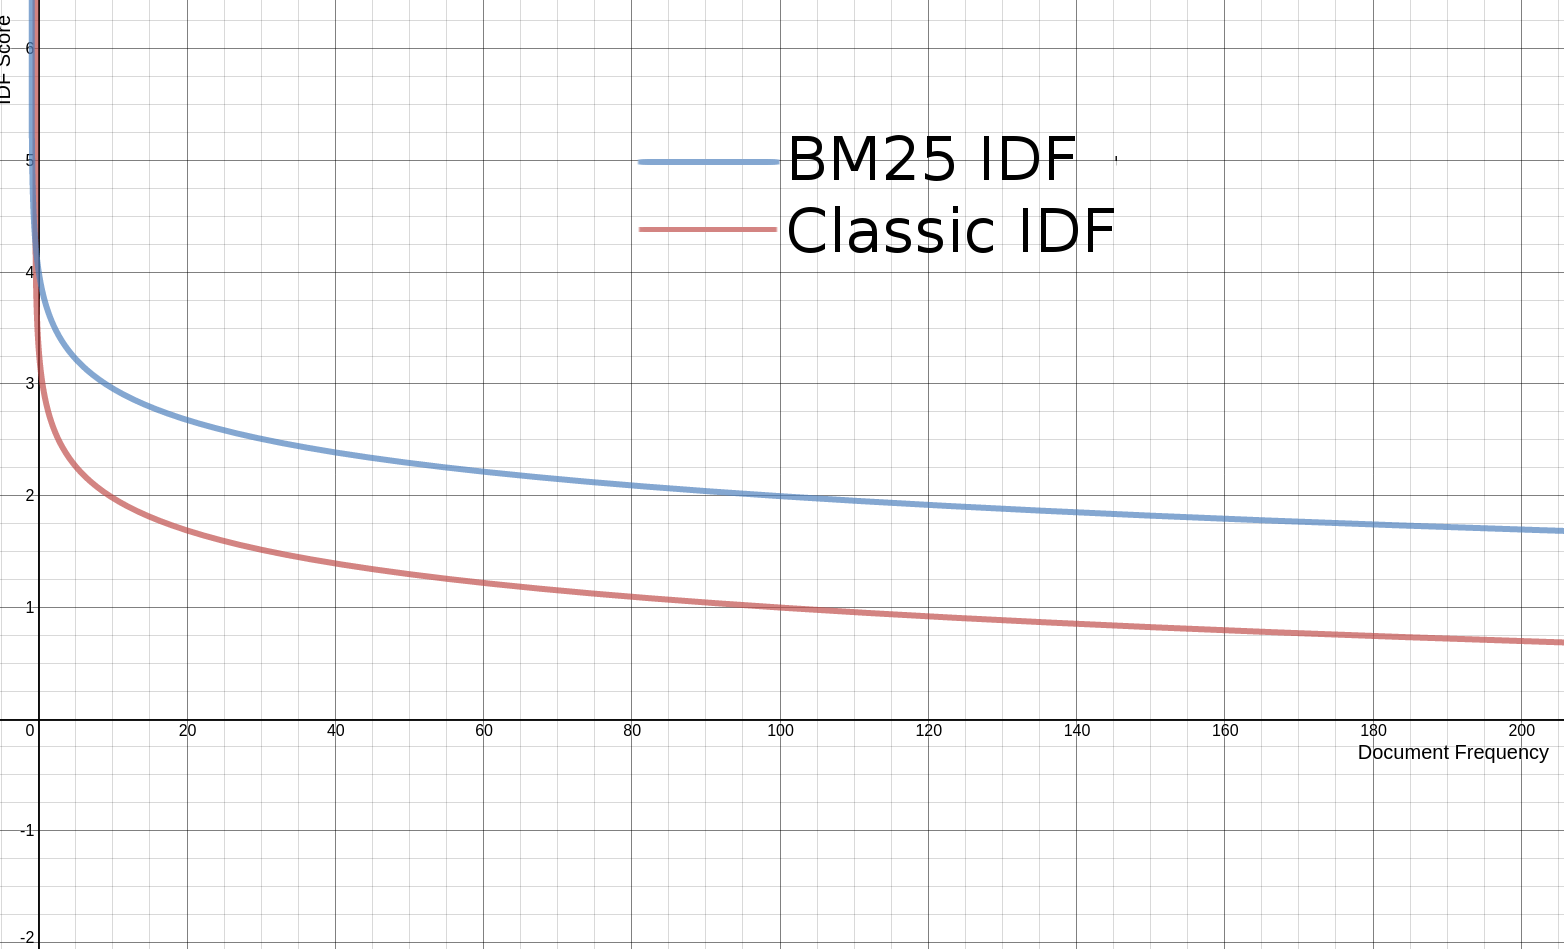
\includegraphics[width=\textwidth]{IDF-comparison-tf-idf-bm25.png}
        \caption{IDF comparison in TF-IDF and BM25}
        \label{fig:IDF-comparison}
    \end{figure}
    Figure \ref{fig:IDF-comparison} shows a comparison of the classic IDF and BM25 IDF. Major change in both the formula is the additional 1. In classic IDF, there are chances of returning a negative values, this is mitigated by use of additional 1 in the log function.
    \item $fieldLen$ denotes the length of present field(or document length) and $avgFieldLen$ denotes the average field length of the entire corpus. 
    $\frac{fieldLen}{avgFieldLen}$ is used in the formula, which calculates the relative length of the present document with respect to the full corpus. The intuition for this is, if the document length is bigger than the average document length, then the denominator becomes large, hence reducing the term weight value. For example, if a term "tiger" appears once in a 200 pages document, then the term might not be significant, however, if the term "tiger" appears twice in a tweet, then it is much relevant about the term.
    \item a constant term $b$, which is multiplied by the field length parameters. If $b$ is large, then the relative length of the document is increased and vice versa. By default, the value of $b$ is 0.75.
    \item $k1$ and $f(q_{i},D)$ are used in both numerator and denominator. Looking at their significance individually,
    \begin{enumerate}
        \item $f(q_{i},D)$ denotes the number of times the term $q_{i}$ appears in a document $D$. This is the same as term frequency used in the TF-IDF formula shown in equation \ref{eq:2.1}.
        The intuition for term frequency is the more number of times a term occurs in a document, more it is relevant to the query.
        \begin{figure}
            \centering
            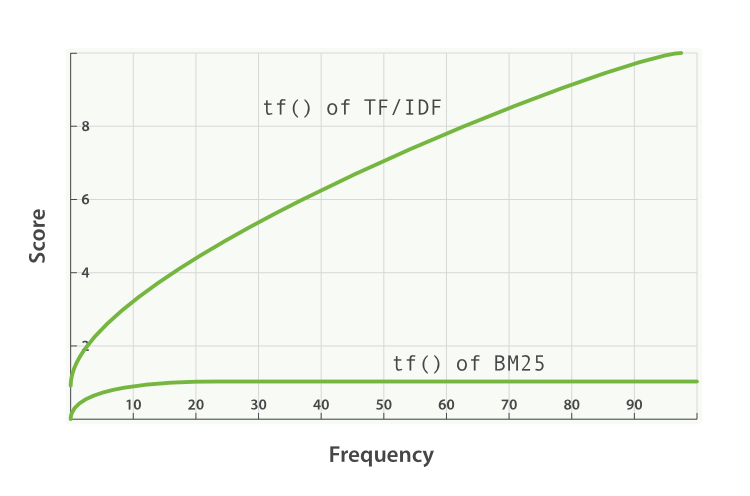
\includegraphics[width=\textwidth]{term_frequency_saturation.png}
            \caption{Term Frequency comparison in TF-IDF and BM25}
            \label{fig:tf-comparison}
        \end{figure}
        \item $k1$ is a constant term to normalize the term frequency $f(q_{i},D)$. This is a new parameter introduced in the BM25 notation. Figure \ref{fig:tf-comparison}  shows the comparison of scores along with term frequency in BM25 and TF-IDF models. This value of k1 can be interpreted as for average length documents, term frequency is approximated to half the actual term frequency of the term. In the figure, we can observe that the score increases rapidly for values where $tf < k1$ and grows gradually when $tf>k1$.
        This k1 value is often set to 1.2. 
        
        
    \end{enumerate}
    
\end{itemize}

\section{Universal Sentence Encoder (USE)}

Universal Sentence Encoder \cite{RN32} is a not specifically a term weighting scheme but a more advanced model used for text embedding into high dimensional vectors and consequently used in tasks such as text classification, semantics, clustering, information retrieval, recommender systems, and other text related tasks.

USE is trained and optimized for more than simple term-based text embedding and works on the sentence level, phrases or small paragraph embedding into a dense vector \cite{RN32}. The USE model is trained on a variety of natural language texts and different data sources to be used in multiple natural language processing tasks. The input is the variable-length English text and the output is a 512 dimension vector. The USE model is trained with a deep averaging network(DAN) encoder \cite{RN32}.
Some of the classic applications of universal sentence encoder are semantic similarity and text classification.
\begin{itemize}
    \item \textbf{Semantic Similarity:} Semantic Similarity shows the level to which two different texts denote the same meaning. This is mainly used to get better results in information retrieval tasks and all related tasks based on understanding natural language. 
    \item \textbf{Text Classification:} Text classification models show better accuracy and efficiency when trained with an enhanced text embedding model such as USE.  Custom binary text classifiers can be trained with the USE model to perform well on the wide variety of classification tasks with a smaller amount of labelled data.
\end{itemize}

The intuition behind USE model is to embed sentence into dense vectors that mark transfer learning tasks to NLP tasks. These models are effectual and result in good performance and accuracy in transfer learning tasks for natural languages. Studies have compared different models implementing word embedding and sentence embedding for trade-offs between accuracy and computational resources. The comparison studies the model complexity, availability of data, and the overall task performance. The comparative analysis shows that the transfer learning along with sentence embedding performs significantly better than the word embedding model and also with a lesser amount of supervised training data availability.

The USE model can be formulated by two methods, first by the use of transformer architecture and the other by the use of deep averaging network(DAN) \cite{RN32}. Both the specified models are implemented using TensorFlow. The input for these models is English strings and output produced is fixed high dimensional vector representation of the same. This sentence embedding can also be used to compute the sentence level semantic similarity. And experiments show the improved performance of sentence based semantic similarity over the semantic textual similarity. Also, the sentence based models can be trained and modified for improved performance in the gradient-based approaches.

The transformer-based sentence encoding model constructs sentence embeddings using the encoding sub-graph of the transformer architecture \cite{vaswani2017attention}. The sub-graph creates the context-aware representations of every word in a sentence that considers the positioning as well as the meaning of other terms in a sentence. These context-aware representations are then converted into a fixed-length sentence encoding vector by summing the representation of each word position. Next, the encoder takes these string tokens as input and returns a fixed 512-dimensional vector. The encoder is designed as a general-purpose model that can be used in a wide variety of applications. This is achieved by using a single encoding model for multiple tasks. These tasks might include, unsupervised learning for arbitrary running text, a conversational input response task for conversational data, and classification tasks to be trained on the supervised model. 

The second approach model used in USE model is based on deep averaging network(DAN); where the average of input word embedding and bi-grams are passed through a feed-forward deep neural network to produce sentence embedding \cite{iyyer2015deep}. 
Similar to the transformer-based approach, this model takes string tokens as inputs and produces a 512-dimensional sentence embedding.
The training method remains the same as in the transformer-based approach. The major advantage of DAN model is that the compute time is linear for the length of the input sequence. This DAN based also shows significant improvement in text classifications tasks \cite{RN32}.

In classic retrieval method, a common way to convert a text into a numeric vector is by allocating a dimension to every word in the vocabulary. The vector is formulated as the number of times the term occurs in the text corpus. This is referred to as the "bag of words" model, based on just the frequency of terms and not sentence structure \cite{julie2019USE}.

There are certain differences in this traditional approach and text embedding model, they are:
\begin{itemize}
    \item text embedding generates are low dimension vector in the range of 100-1000, whereas the bag of words generates a more sparse matrix with much higher dimensions. This is because embedding model considers semantic context and words with similar meaning will have the same vector representation.
    \item Sentence embedding model considers the order of terms while defining the term vectors. For instance, "tune in" will be given a different vector compared to "in tune". \cite{julie2019USE}
    \item also, sentence embedding model (USE) cannot represent the semantic context for a larger section of text. And can be used only for smaller sentences and phrases.
\end{itemize}

From search and information retrieval perspective, this Universal Sentence Encoder model is incorporated as follows:
\begin{itemize}
    \item all the documents in the corpus are run through pre-trained sentence embedding model to generate its respective dense vector of a given dimension.
    \item similarly, the user query is also run through the same sentence embedding model to produce a numeric vector. And then the similarity between the input query vector and the documents vector is calculated using cosine similarity given in \ref{eq:2.4}
    \begin{equation} \label{eq:2.4}
    \cos \theta = \frac{\sum_{1}^{n} \vec a_{i}b_{i}}{\sqrt{\sum_{1}^{n} \vec a_{i}^2}\sqrt{\sum_{1}^{n} \vec b_{i}^2}}
\end{equation}
\end{itemize}
  
\chapter{Related Work}

	\section{Term Weighting Modifications}
	TF-IDF is a relatively old approach and there have been many studies comparing the results of TF-IDF with other states of the art term weighting schemes. Also, different researches have suggested novel variants and enhancing algorithms solving various issues. For instance, \cite{RN23} points out the lack of personalization in classic TF-IDF. The authors have highlighted the issue of access to the document corpus for calculating IDF, that is not always available and another issue of ignoring the information from the user’s document collection for recommendations and user modelling. The problem also relates to the concept of frequency distribution in standard TF-IDF. Since the TF and IDF values are calculated based on the occurrence of the same term in other documents as well, so the assumption is that the term is relevant in other documents as well. However, this might not be true, especially in cases of creating user models. Thus, a novel term weighting is suggested, that does not require the document corpus and uses the user’s document collection for user modelling. The term weight formulation in this algorithm is formed by two components, first is TF, which is same as the one in the classic algorithm, that marks the document more relevant based on the high frequency of a term in a document. The calculation for IDF is different from the classic one and is termed as IDuf, that is user-focused and is calculated using the document frequency from the user's collection. And higher relevance is given to the terms that occur less frequently in the document collection.

	In another paper, \cite{RN24} points out the problem of using IDF in text classification. The basic idea behind IDF is that a term occurring frequently has negligible distinguishing power, however, in the case of text classification, this might not be true, because, highly frequent terms in different documents of the same category can be helpful in text classification. Hence, the authors suggested two variants using the supervised learning approach. In one of the approaches, the authors calculate the IDF excluding the category to be considered. In the second approach, the first approach of calculating the IDF is combined with relevancy frequency that considers the category under analysis. However, this model is built out for term weighting in text classification applications and needs to be extended to other fields.
	
    \cite{tian2010improvement} suggested an improvised version of TF-IDF by introducing term distribution. The authors have highlighted the issue of non-reliability on the term frequency since that is based on a single document and cannot be used to as stable differentiating factor between terms and documents.
    To mitigate this issue, the authors have studied different statistical characteristics of terms and suggests the algorithm based on term distribution along with the term frequency. The interesting part of this research is the relation of term distribution with term frequency leads to semantic similarity within documents. Results shown in this paper indicate the significance of term distribution on both the TF and IDF values.
    A similar concept has been used in our research of using term age along with the term weight values to study the similarity of documents with the given topic.


	\cite{RN26} suggests a novel approach to term weighting based on the term positions along with the TF and IDF terms. This research points out the problem of ignoring the term position in the existing retrieval methodologies. Some researches such as  \cite{clarke2000question} have studied the proximity methods for similarity function and suggested that thee documents having small proximity within the query terms are more relevant for the given query. The authors in  \cite{RN26} have extended the same hypothesis and studied the term patterns that occur in the documents using the wavelet transform method. The wavelet transforms breaks the input signal into small waves of different measure and positions. This disintegration of wavelet analyzes the signal at distinct frequency resolution and trace any variation in the position in the signal. This method is usually used in image processing for studying colour variations. A similar approach is used with the stream of text in this case. The low-frequency wavelet represents the scattered terms in a document with a high term frequency and a high-frequency wavelet is used to represent a term that occurs less frequently in the document. With the help of this system, this research shows the wavelet transform method helps in attaining high precision and fetches the results faster with a condensed index. 
	Another contribution of this research is the study of term occurrence patterns. The authors have implemented different types of retrieval methods such to study term patterns, such as Spectral-based document retrieval, and Vector space retrieval. And a comparative analysis of the proximity methods and spectral based retrieval is shown suggesting the low latency in spectral approach. Finally, the research infers that the documents are ranked more relevant if the query terms are close to each other.
	
	In all these researches, we see the authors have tried to fix a flaw in the existing term weighting methodologies. The major idea that we get out them is the existing metrics like term frequency and inverse document frequency are not sufficient to consider different contexts and deal with all different types of use cases that we try to solve from term weighting. This gives us a start in the direction of enhancing the existing term weighting schemes for our research objective.

	\section{Time Aware Models}
	Recommendation system works up to suggest the items to users based on their past choices. For building up such a system, different contexts such as location, time, weather, etc. play a major role, in providing efficient recommendations \cite{adomavicius2011context}. Out of these contexts, time is one of the most useful contexts to track the evolution of user searches and preferences. Utilizing temporal feature has also proved to be an efficient way for recommenders for instance in the Netflix Prize contest and time normalized recommendations are certainly receiving growing application in recent times \cite{RN28}. Major applications for the time-based system in user modelling and recommendation engines have been proposed. The authors have critically analysed the concept of time context in recommendation systems and study the different representations of time. For example, time can be considered as a continuous variable as in the case of when was a particular item searched on a particular site or it can be considered a categorical variable such as season of year, summer, winter, autumn, spring. The best way to exploit all these use cases is to store the exact date and timestamp of the activity that can further be utilized in any kind of recommendation system. Other sources of time factor collection come up from data storing the time of purchase, registration time on a site, etc. These timestamps can be mapped to a particular action or event and then used to form the user model based on the temporal context.
	
	
	Another research \cite{7817104} leverages this concept of using timestamp with event summarization on social media. The authors have proposed a variant of TF-IDF, where previous knowledge of the entire dataset is not needed to get the term weights. The intuition behind this approach is that if a term occurs more frequently over a specific period, they are given higher weighted compared to the ones that occur less frequently. In this research, the authors have highlighted the issue of prior knowledge of entire dataset for calculating standard TF-IDF. This causes the issue in cases when it's streaming data and the weights need to be updated frequently in intervals of specific time frames. For such a scenario, it is suggested to consider the iterative calculation strategy for term weights. Temporal TF-IDF approach considers a set of posts in a cluster that represents a document. And the number of clusters is equal to the number of documents in the corpus. The advantage of this approach is it reduces the computational load on the system and also overrules the need to know the entire corpus at once for calculating Tf-idf. With the cluster of posts, the timeframe is tagged along with it, and that adds not only for the current timeframe but also for the previous timeframe to make the weight distribution more dynamic and relevant to the user. This part of considering two timeframes for computing term weights also helps in relative term weighting and marks the documents more relevant based on the high frequency of occurrence over a specified time frame.
	
	
	One of the researches \cite{RN27}, that falls closest to our research objective, suggests usage of time-normalized term weighting for user modelling. The main aim of this search is to enhance the user experience by building out personalized search results. In the current age scenario, with an expanded usage of the social web interactions, personalized search engines are based on the extraction of user preferences and interests. The intuition in this research is based on the fact that a user's interests change over time, so the personalization of search results should not only be based on the content of the search but also on the time of the search. This bridge of term weight and a user model is filled by using the vector space model, where user preferences are represented as a vector or vectors of keyword and the weight for these keywords are assigned using TF-IDF model or a similar term weighting scheme. It is observed from the weighting schemes that the weights are designated based on the spatial frequency distribution of the keywords without contemplating the diverse factors of them and the user preferences. For instance, suppose a user was living in London for the past many years, and the entire search history is based on London based results and searches. But the user has recently moved to Dublin and has not done much search post moving. In this case, a user model for personalized search would be based on London search history. However, at the moment, a suggestion based on Dublin would be more relevant. In this example, the context of location and time, both play a crucial role in personalization. The research paper \cite{RN27}, considers the elimination of a similar problem by introducing a temporal feature to the term weighting methodology for user modelling. The authors have used the time of social/web search of terms to form the short and long-term contexts and further creating a user profile based on the same. Short term session includes just the current session and the personalization based on the recency and relevancy of recommendations. Long term sessions consider the combination of multiple search sessions.
	
	The main aim of this research is to study the effect of temporal dynamics in user model quality for personalized search framework. And the contribution of this research is the proposal of a personalized search framework, that forms the user model based on the user's web and social media activities. This is done by representing the search interests as weighted term vectors. And the personalized search results are based on both the recency, frequency as well as the persistence of the search keyword.  The comparative study of this algorithm with the standard TF-IDF suggests a significant improvement in results centred on the time normalized user models. Considering this research of temporal context’s effect on term weights, we propose a Time Normalized term weighting algorithms for information retrieval and recommender system, discussed and implemented in this paper.
  \chapter{Time Normalized Term Weighting}
In this chapter, we introduce the novel algorithm of this research, that is time normalized term weighting. In the standard term weighting methodologies, the terms are weighted based on their spatial distribution rather than on the other crucial factors. Consider an example of two terms "COVID19" and "neural networks". Both the terms represent very different meaning and have a different origin year. "COVID19" is a relatively new term being used since last year, while "neural network" is being used since decades. However, term weighting schemes will weight the terms based only on their frequency distribution, no matter what. In this paper, we try to emphasize on the importance of term recency in relevant results retrieval. The premise for this algorithm is that, if a term is devised newly then there are probably a lesser number of documents containing the term compared to the term which is being used for a longer duration of time. Considering both the aspects of origin year and document frequency, in this algorithm, we introduce a term recency factor along with standard metrics to compute the term weight. The formulation and implementation of the algorithm is further explained in this chapter.

We have also presented this novel algorithm at the WOSP workshop \footnote{WOSP 2020: https://wosp.core.ac.uk/jcdl2020/index.html}, and will be published in the proceedings of the conference. This serves as a contribution to the research community to use this algorithm and can also be extended for further research.

\section{Term Age Calculation}
The time based factor(can also be referred as Term age) is formulated from the origin year of the word(can be from different sources) and the document frequency of the term, computed as the ratio of both giving the metric as documents per year. For a given term $w$ in document $d  \epsilon D$, where $D$  is the document corpus $D$ with size $N$, term-age is calculated as:
\begin{equation}
    t_{w,D}=\log(df_{w,D}/(y_{diff}+1))
\end{equation}
where $y_{diff}$ is calculated as :
\begin{equation}
    y_{diff} = y_{current} - y_{origin}
\end{equation}
where $y_{origin}$ is the year of first usage of the word and $Y_{current}$ is the present year.

We have not considered the article publishing year and take current year for certain reasons. Since a term can be used in multiple years, so the age calculation would change every time and choosing either of them would be a tough call. Also, this might result in certain anomalies and ambiguities in the age calculation. To simplify this logic and to have the same age for a term across the corpus, we consider the current year, which is the last year of articles published in the corpus. We take the logarithm of the terms to normalize the value, since this can go to a large number based on the size of the corpus. Also, we take up the absolute value of log, so that we don’t have negative weight values. 1 is added in the denominator to avoid the divide by zero error in case if the origin year is same as the current year. 

The $y_{origin}$ can be traced from multiple sources depending on the problem statement. Considering few examples, and the formulation of term age factor respectively:
\begin{itemize}
    \item if a research paper recommender is being developed, the origin year can be retrieved from the year of first occurrence in a research paper. And the current year can be the last year of the article/paper present in the corpus.
    \item in case of web based personalized search engine, time of first search of the specific term can be used to form the temporal context as used in \cite{RN27}. The difference from the first usage year to the current year can be used as the year difference.
    \item for a more generic instances and to make the calculation more robust, the origin year can be traced to the etymology and the year of first occurrence can be fetched. This can also be used to fetch other contexts of the word based on the word origin, and usage to improve search results and recommendations however, these aspects are beyond the scope of this research.
\end{itemize}
In our research hypothesis, we have used the origin year as the generic one and fetch it from etymonline.com to get the etymology and fetch the year of first occurrence. We have used the news dataset \cite{RN20}, that have terms being used which explain a wide range of temporal context. We have also tested the same algorithm on research paper dataset \cite{DBLP:conf/ijcai/WangCL13} and a web answer retrieval dataset \cite{RN30, RN31}. And also to keep the algorithm more robust and generic, testing the etymology seems to be an apt way to test the hypothesis. We have introduced the term age factor in three of the term weighting schemes, that is TF-IDF, BM25 and USE, explained in the following sections.


\section{Time Normalized TF-IDF(tTF-IDF)}
TF-IDF is the classic term weighting methodology, that weights the terms based on two factors, term frequency and inverse document frequency. Both these factors are based on the spatial distribution of terms that is the frequency of their occurrence in the corpus. This formulation is shown in Equation \ref{eq:4.3}
\begin{equation} \label{eq:4.3}
        wt_{w,d} = tf_{w,d}*log(\frac{N}{df_{w,d}})   
\end{equation} 
The real issue in this formulation is that, the TF-IDF assumes that a frequency distribution remains constant over time. In short periods of time, this holds true, however, over longer periods of time, this assumption fails. To overcome the issue that terms have temporal distributions of frequency not just space distribution, which are unaccounted when using TF-IDF, we proposee the time normalized TF-IDF. This is computed as shown in equation \ref{eq:4.4}.

\begin{equation} \label{eq:4.4}
        wt_{w,d} = t_{w,D}*tf_{w,d}*log(\frac{N}{df_{w,d}})   
\end{equation} 

With the introduction of term age factor, we intend to incorporate the temporal context of the terms for an improved search results.

\begin{figure}
    \centering
    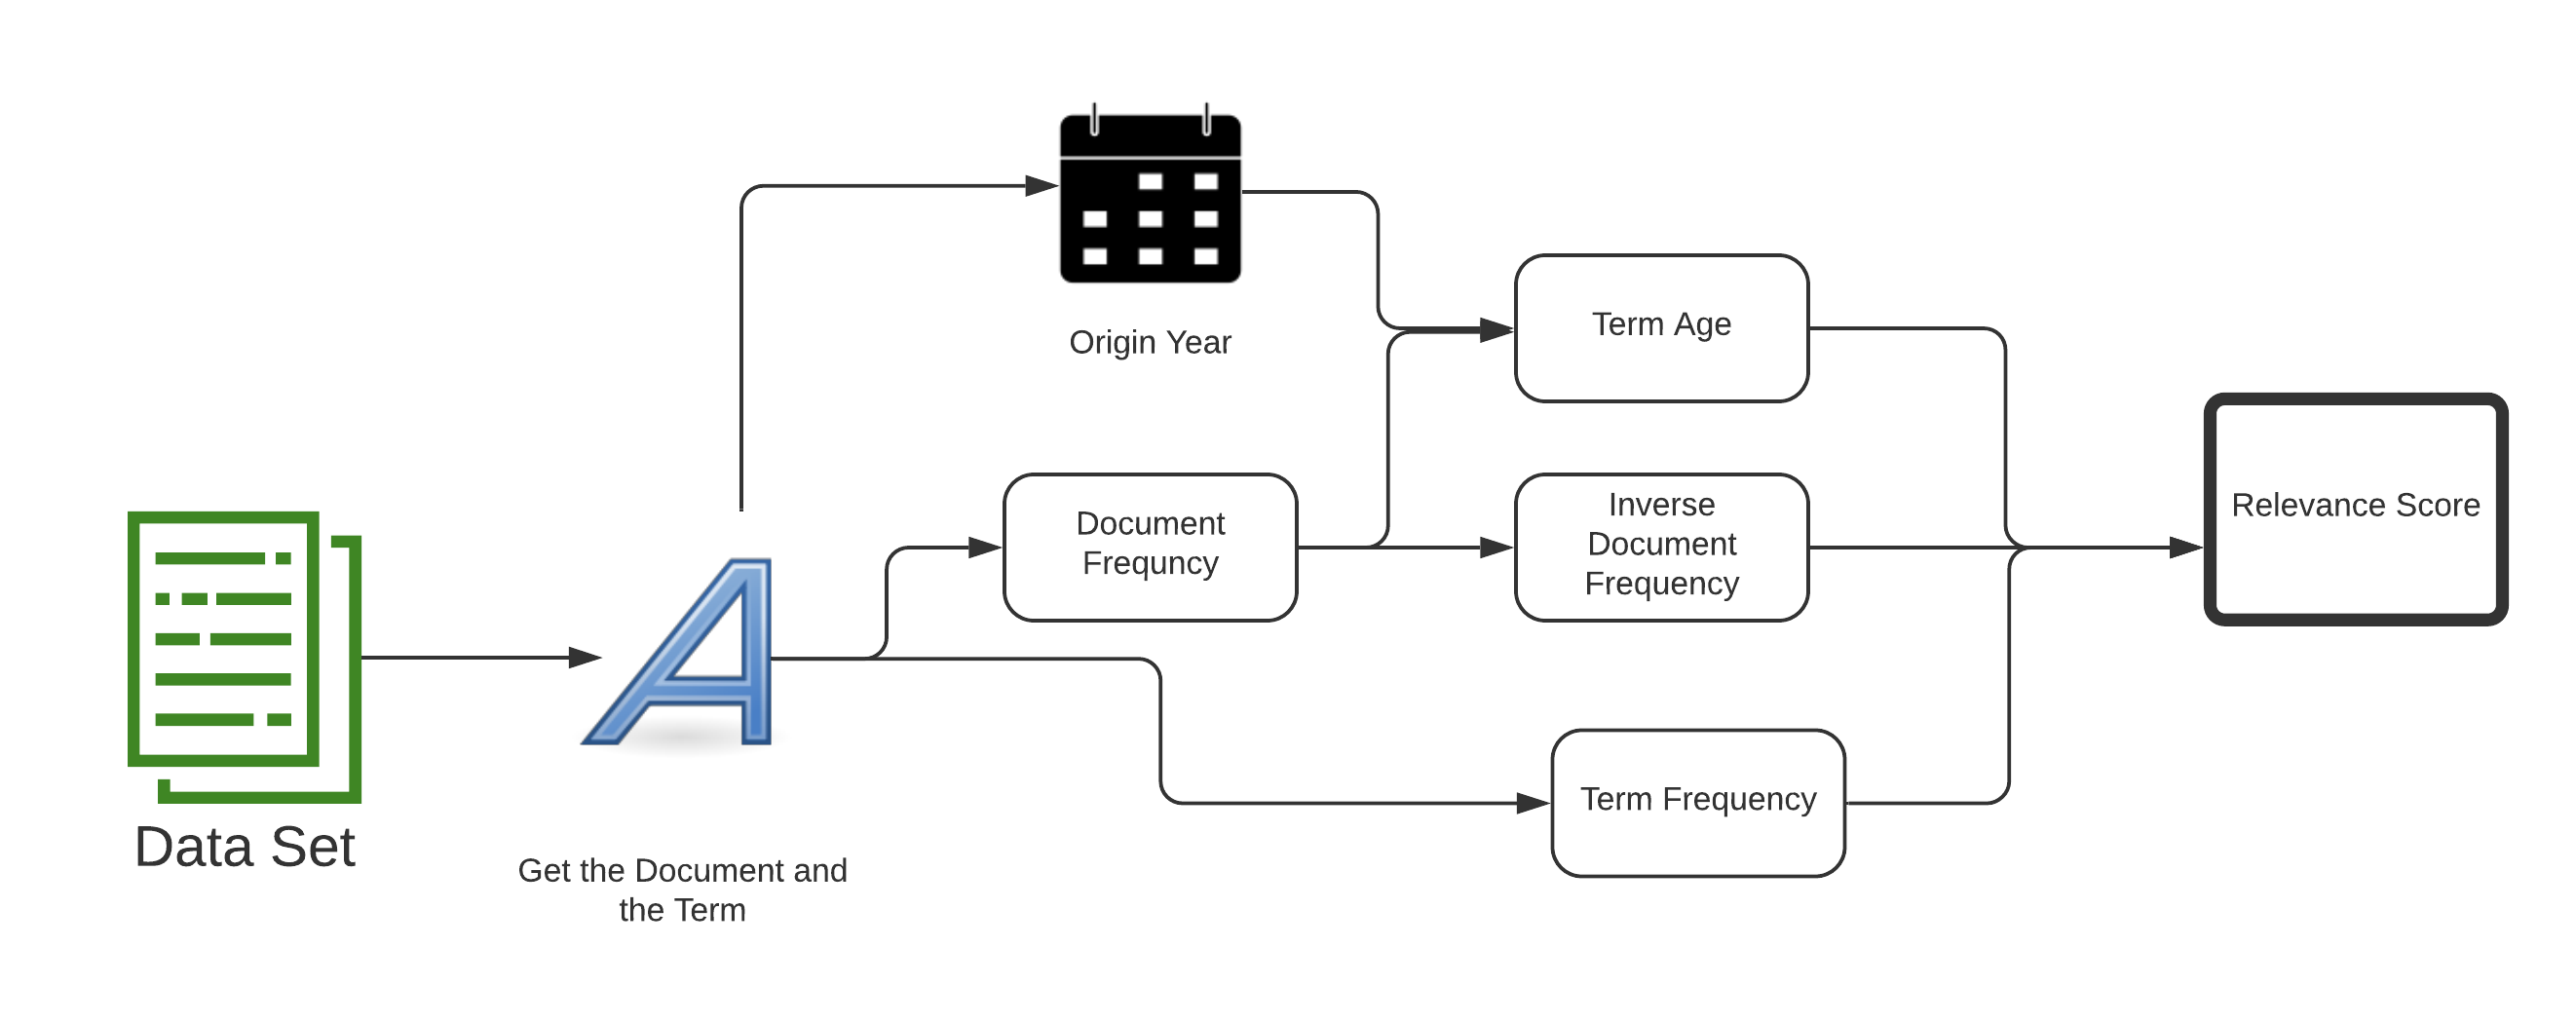
\includegraphics[width=\textwidth] {algorithm-working.png}
    \caption{Algorithm Working for tTF-IDF }
    \label{fig:tTF-IDF-working}
\end{figure}

\section{Time Normalized BM25(tBM-25)}
BM25 is another standard term weighting methodology that is also based on term frequency and inverse document frequency calculations, but the logic to calculate these metrics changes. IDF is calculated the same way as in the TF-IDF but with an added 1 in the denominator to overcome the divide by zero error. For computing the term frequency, some additional term based metrics such as field length and average field length are considered. Some other constants such as k1 and b are also considered in this formula, that are used to normalize the term weighting scores. This formulation is shown in Equation \ref{eq:4.5}.
\begin{equation}  \label{eq:4.5}
    wt_{w,d} = \sum_{i}^{n}IDF(q_{i}) * \frac{f(q_{i},D)*(k1+1)}{f(q_{i},D)+k1*(1-b+b*\frac{fieldLen}{avgFieldLen})}
\end{equation}
Although this overcomes the issues found in the TF-IDF and performs better in some cases, but the issue of not considering the diverse context of the term in various aspects still remains the same. Even the added metrics such as field length and constants k1 and b, are all based on the spatial distribution of the terms. As we formulate the tTF-IDF, similarly, we deduce the formula for tBM25 introducing the term age in the term weight calculation. This formulation is shown in Equation \ref{eq:4.6}. And this time-normalized term age factor works on to consider the temporal aspect of the terms as well.
\begin{equation}  \label{eq:4.6}
    wt_{w,d} = \sum_{i}^{n} t_{w,D}*IDF(q_{i}) * \frac{f(q_{i},D)*(k1+1)}{f(q_{i},D)+k1*(1-b+b*\frac{fieldLen}{avgFieldLen})}
\end{equation}
\section{Time Normalized USE(tUSE)}
Universal Sentence Encoder(USE) is not specifically a term weighting methodology but a more advanced scheme. Text embedding and sentence embedding model convert the given text into high dimensional vectors and then the similarity between these vectors is mostly calculated using the cosine similarity function. This cosine similarity finds the angle between the given vectors and the lesser the value of the angle, more similar the texts are. This formula for finding the cosine similarity between the high dimensional vectors is given in Equation \ref{eq:4.7}.
\begin{equation} \label{eq:4.7}
    \cos \theta = \frac{\sum_{1}^{n} \vec a_{i}b_{i}}{\sqrt{\sum_{1}^{n} \vec a_{i}^2}\sqrt{\sum_{1}^{n} \vec b_{i}^2}}
\end{equation}
The main advantage of using the USE model in the text retrieval task is that it considers the semantic context of the text along with frequency distribution. This performs well in most of the text based searches and gives pretty good results in our datasets as well. However, the issue we are addressing in this research still remains missing in the formula logic. Similar to other two term weighting methodologies, we have multiplied the term age factor with the regular cosine similarity function for text similarity and get the updated version as tUSE. This computation is shown in equation \ref{eq:4.8}.
\begin{equation} \label{eq:4.8}
    \cos \theta = t_{w,D}*\frac{\sum_{1}^{n} \vec a_{i}b_{i}}{\sqrt{\sum_{1}^{n} \vec a_{i}^2}\sqrt{\sum_{1}^{n} \vec b_{i}^2}}
\end{equation}
\section{Algorithm Analysis}
As we can see the term age is not only dependent on the origin year but also the number of documents the term occurs in(document frequency). This can also be considered as an added factor to the IDF value, but with a different significance. Let us consider the impact that document frequency and time difference have on the term weight value. Now, assume that a term is new and occurs in reasonable number of documents, then the value of term-age, $t_{w,D}$ will be large and hence the term weight will be large.
And contrast case if the term is relatively new, and occurs is lesser number of documents, that is an expected behaviour that the term would be weighted low due to its lesser significance value.
Similarly, if the term is being used for many years and is occurring in many documents, it will relatively reduce the value of the time-factor, thus giving it low importance. 

A caution which needs to be taken while implementing this algorithm is to check for more commonly occurring non relevant terms which are normalized by using IDF should not get boosted. For example, occurrence of stop words, these occur maximum number of times in any corpus, and are irrelevant in general search retrieval schemes. This can be taken care of while calculating the value of $y_{origin}$, and such terms can be ignored so they don’t boost up the term weights based on non-relevant terms. Or if the stops words don't have much significance even in the semantic logic of the retrieval system, they can be removed in the first index itself. That will save the computation as well as reduce the chances of unwanted partiality in the results.

  \chapter{Methodology}
\section{Datasets Description}
\subsection{TREC News Dataset}
\cite{RN19} This collection contains 608,180 news articles and blog posts ranging from January 2012 to August 2017. For the purpose of testing our hypothesis, we use a sample of $\mathtt{\sim}$ 21000 documents with approximately $\mathtt{\sim}$ 2400 relevant documents. However, this has been done only for time-based index due to scalability and resource constraints. And the term age is still calculated considering the entire corpus and does not affect the algorithmic logic. The dataset is in JSON file format containing following fields: id, URL, title, author, published date, article text broken into paragraphs, caption and author bio. We have created three indices in our Elasticsearch server, one which contains all this dataset, as present in the given JSON file, with a regular mapping. Second index containing the updated term weight parameter containing a time normalized term weight to be used later in relevance score calculation and retrieval. And a third index containing the USE text embedding vector field along with the term weight parameter.

For testing the results, and setting up a ground truth for the system, we have used TREC – 2018 news background linking task \cite{RN20}. This task is about fetching the background related news articles providing the context for the main article. The intuition behind this is the reader should get all the relevant information about the searched topic from the best possible source \cite{Huang2018trec}. For example, if the search topic headline is "How major U.S. cities and transit systems are reacting to the Brussels attacks", then the related relevant article would be "Transportation agencies across the U.S. step up security in wake of Paris attacks" or "Islamic State claims responsibility for the Brussels attacks". There are 50 such queries given to us, with the following fields, Document number, ID, URL. This is used as an input query file to our information retrieval system. Another data file is given which contains the most relevant results for each given query in the input document. These results are human checked and can be considered as the ground truth for our experiment. This file contains the following fields: Document Number, Document ID, Gain Value (which is defined as $2^r$, where r is relevance scale ranging from 0 to 4). Document number referred in this file is same as the one given in the input queries file. So, this file sets up the ground truth for the given set of queries, the documents which are relevant to each query and scale of relevancy for these documents.
\textit{Figure} \ref{fig:trec-news-dataset} shows the glimpse of the dataset and its structure and \textit{Table} \ref{tab:trec-ground-truth} shows the relevant gold standard relevance values given to us.

\begin{table}[h!]
    \centering
    \begin{tabular}{|c|c|c|}
    \hline
    \textbf{query number} & \textbf{id} & \textbf{Relevance ($2^r$)}\\
    \hline
    321 & 00f57310e5c8ec7833d6756ba637332e & 16\\
    321 & 02ae7136-006d-11e3-9711-3708310f6f4d & 2\\
    321 & 049739753ce2e539d8dc2165daaf6aa6 & 4\\
    \hline
    \end{tabular}
    \caption{TREC News gold standard snapshot}
    \label{tab:trec-ground-truth}
\end{table}

\begin{figure}
    \centering
    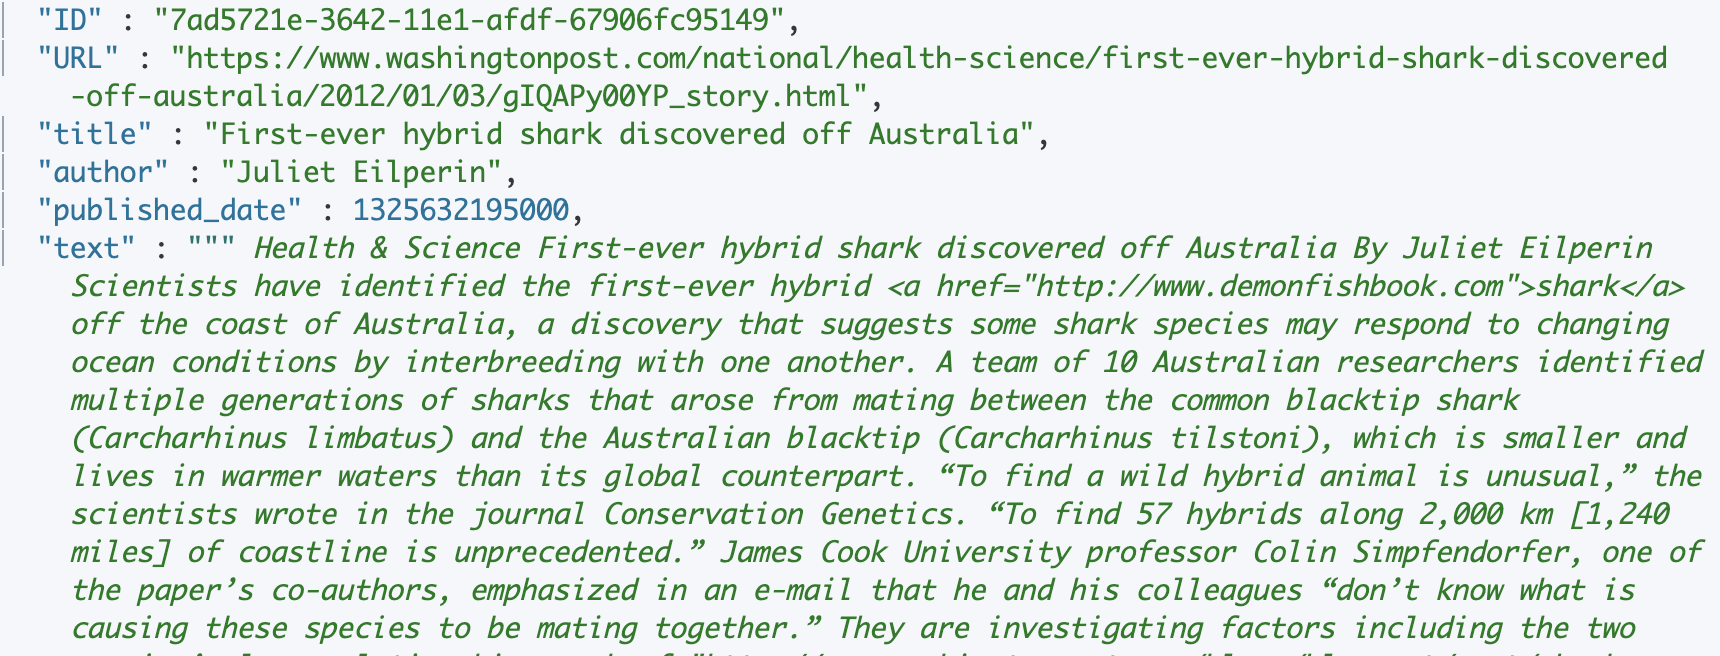
\includegraphics[width=140mm, scale=0.7] {trec-news-dataset-structure.png}
    \caption{TREC News dataset structure }
    \label{fig:trec-news-dataset}
\end{figure}

\subsection{Web AP Dataset} 

\cite{RN30, RN31} This collection contains 8027 articles from the web, which are answers to 82 TREC queries. The dataset is a subset of 2004 TREC Terabyte track Gov2 dataset \cite{clarke2004overview} along with the test query topics specified in the track. This dataset is cleaned and contains relevant passages for the 82 test queries specified in the ground truth. Length of an average passage in this dataset is 45 words.
\begin{figure}[h!]
    \centering
    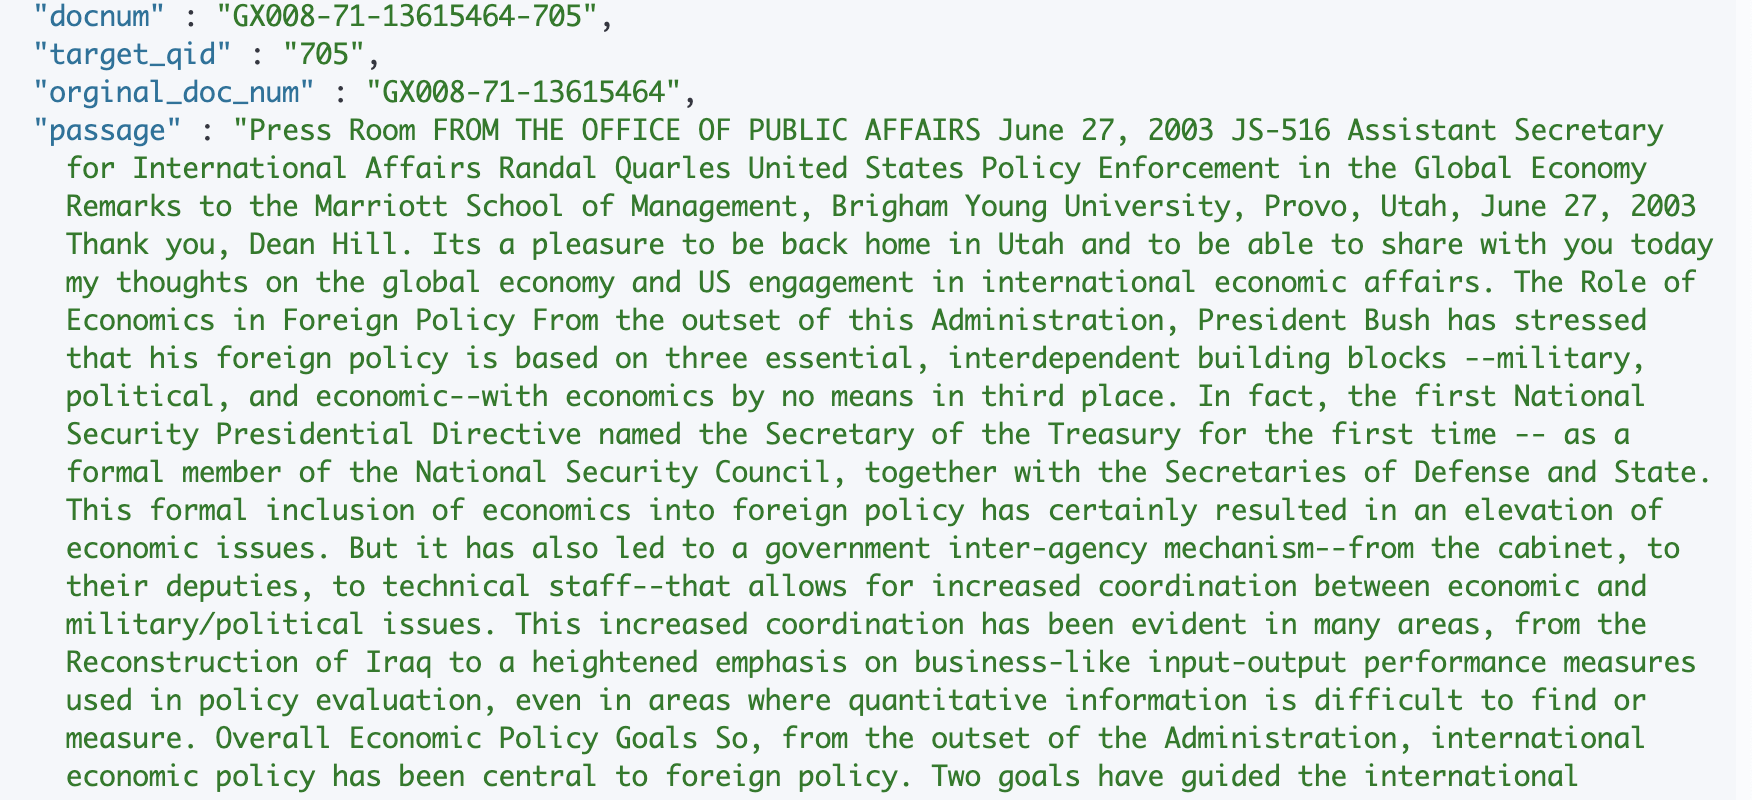
\includegraphics[width=140mm, scale=07]{WebAP-dataset-structure.png}
    \caption{Web AP dataset structure }
    \label{fig:web-ap-dataset}
\end{figure}

The dataset is in JSON file format containing the following fields: unique document id, target question id, and passage. We have created three indices from this dataset, one containing the data as it is given in JSON file. Second index containing the updated term weight parameter as the time-normalized factor. And the third index with dense vectors for USE embedding along with the time-normalized factor. We are given ground truth results for the given set of 82 queries as set of 50 most relevant results. The results are given as question\_id, document number and relevance as ranked from 1 to 50. \textit{Figure} \ref{fig:web-ap-dataset} shows the glimpse of the dataset and its structure.

One of the sample query used in the evaluation is given in the following form: \\
\textit{
$<$query$>$	\\	
$<$title$>$\\	
$<$docno$>$DOCNO701$</$docno$>$.\\
$<$tag$>$U.S. oil industry history $</$tag$>$\\
$</$title$>$\\	
$<$desc$>$\\	
$<$docno$>$DOCNO701$</$docno$>$.\\
$<$tag$>$ Describe the history of the U.S. oil industry $</$tag$>$\\
$</$desc$>$	\\
$</$query$>	$\\	
}

And table \ref{tab:web-ap-gold} shows a snapshot of the gold standard relevance results for the above mentioned query:
\begin{table}[h!]
    \centering
    \begin{tabular}{|c|c|c|}
    \hline
         \textbf{Number }& \textbf{docnum} & \textbf{relevance}  \\
         \hline
         701 & GX268-35-11839875 & 1\\
         701 & GX262-28-10569245 & 2 \\
         701 & GX238-57-4348848	& 3	\\
         701 & GX231-53-10990040 &	4\\	
         \hline
    \end{tabular}
    \caption{Web AP Gold standard relevance}
    \label{tab:web-ap-gold}
\end{table}


\subsection{CiteULike Dataset}
\cite{DBLP:conf/ijcai/WangCL13} This dataset is collected from CiteULike and Google Scholar and contains 17013 documents. CiteULike was a service that allowed people to create their personal article or paper collection. The dataset is given in CSV file format with the following fields: docid (unique document id), title (lower case title), raw\_title(original title of the research paper), and abstract. We have created three indices from this dataset, one containing the data as it is and another one containing the time normalized term weight parameter and a third index containing the dense vectors based on USE encoding along with the term age metric.

We are given another file in this dataset, that contains the referenced articles for every document. This serves as our problem statement to develop a research paper recommender system. The input for this will be the title of the paper and the expected results would be the referenced article for this paper. Since the references are given for every article, and it will make the evaluation biased and difficult for aggregating the results. In order to fix this issue, we have randomly selected 116 test topics having exactly 10 citations to be used as our ground truth. 
\textit{Figure} \ref{fig:citeulike-dataset} shows the glimpse of the dataset and its structure.

\begin{figure}[h!]
    \centering
    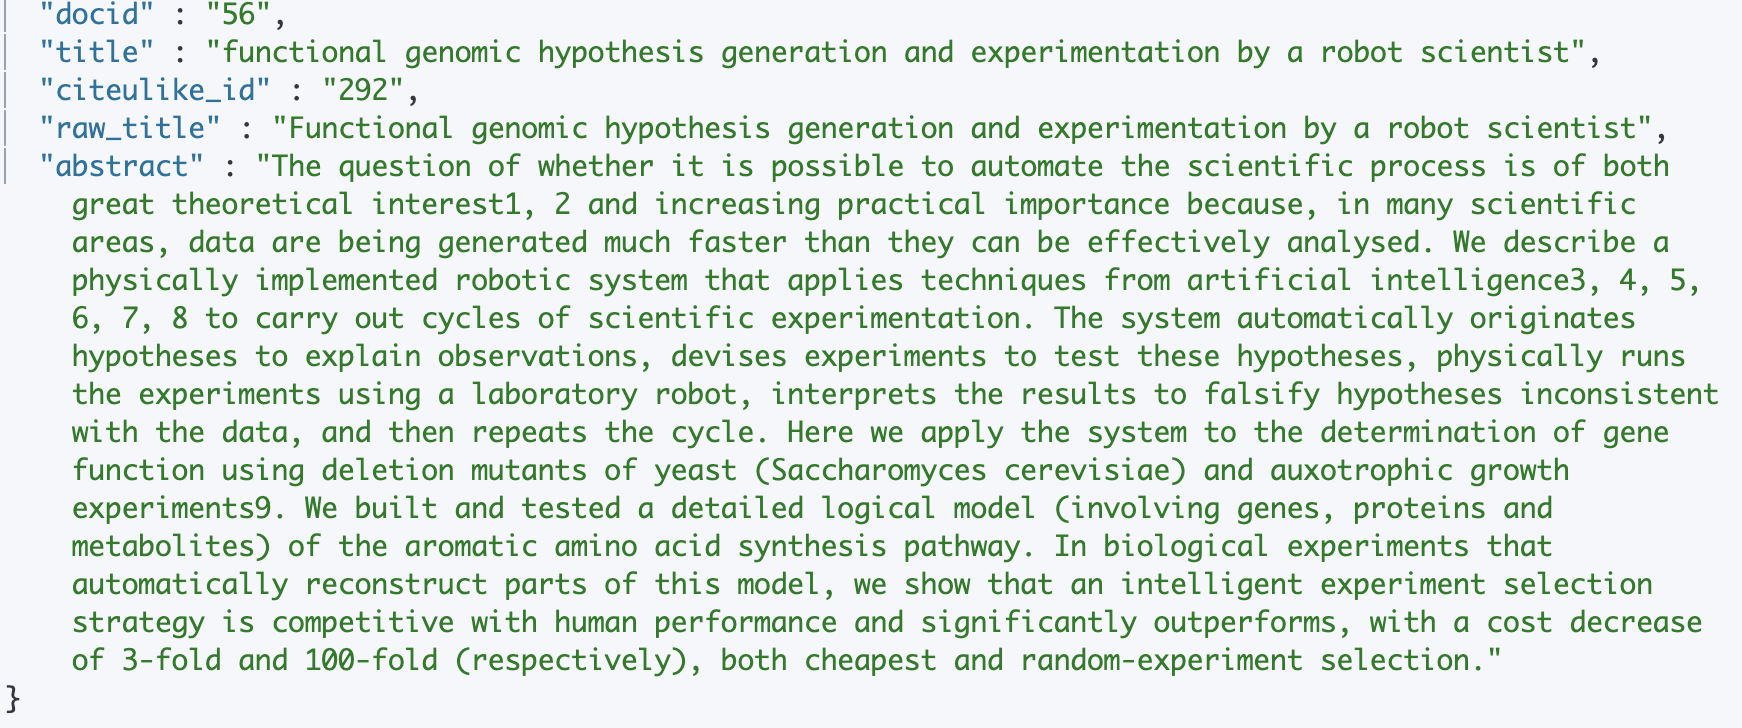
\includegraphics[width=140mm, scale=0.7]{cite-u-like-dataset-structure.png}
    \caption{CiteULike dataset structure }
    \label{fig:citeulike-dataset}
\end{figure}

\section{Evaluation Metrics}
\subsection{Precison@10}
Precision is defined as the number of relevant results in retrieved result set. Generally, precision is calculated for top K number of results, given as P@K. This evaluates the number of relevant results fetched in the top K number of results. We have tested our IR system on given set of 50 queries(for TREC News), 82 queries(for Web AP) and 116 queries(for CiteUlike) , so we calculate the average precision which takes the mean of the precision calculated for all the given queries. We have taken the value of K as 10, so we test the relevance of top 10 results in our scenario. We have calculated the precision value for top 10 fetched results on the given set of input queries and take an average of the results for comparison.
We have calculated the precision value for top 10 fetched results on the given set of input queries and take an average of the results for comparison.

\subsection{Recall (TREC News dataset only)}
For calculating the recall, we have considered the queries having less than 100 results, in case of TREC news. And then recall is calculated as the number of relevant retrieved document divided by the number of relevant documents present in the index. For other datasets, since the number of relevant results is fixed, so the value of precision and recall remains the same.

\subsection{F1 Score (TREC News dataset only)}
Since F1 score uses both the precision and recall values, so for calculating the precision scores, we have used the same results from the recall measure and used a fixed denominator as the number of retrieved results (100 in our case). Formula used for F1 score is given as:
	\begin{equation}
	    F1= 2*(Precision*Recall)/(Precision+Recall)
	\end{equation}
   
\subsection{NDCG@10 Score}
This is a measure of ranking quality. This is based on the assumption that more relevant documents are placed higher in the result list. In calculating DCG, higher relevant result placed at a lower position is penalized by the log value of proportional to the position. DCG is calculated at specific rank position p, given by 
	\begin{equation}
	DCG_{p} = \sum{i=1}{p} rel_{i}/\log_{2}(i+1)
	\end{equation}
where, $rel_{i}$ is the relevance score of a document at position $i$. And NDCG is calculated by considering the DCG of ideal order along with the DCG values and is given by
\begin{equation}
    nDCG_{p} = DCG_{p}/IDCG_{p}
\end{equation}
where $IDCG_{p}$ is the ideal DCG values at position p. This is considered from the ground truth or from human verified results, that specify the ranking of results they prefer for relevance.
We have taken the value at position 10 and calculated the nDCG for the top 10 results. We have fetched the results for given set of queries, so we calculate the average nDCG for both set of algorithms and compare the results.
  \chapter{Implementation}
\section{Data Indexing}
Data Indexing is the first step in implementing an Information Retrieval system and is crucial for efficient retrieval. The brute force method of document retrieval is the linear scanning of the entire database. To avoid linear scanning, data indexing comes into the picture. For effective indexing and retrieval, both the query and data are expected to be in index form \cite{7830087}.
Data Indexing takes place in four steps: first is the data collection and managing the data corpus, second is parsing the document list, third is tokenizing the terms in the document and create a logical structure, and final step is to create the data index \cite{7830087}. This process of indexing is shown in Figure \ref{fig:data-indexing}. 

\begin{figure}
    \centering
    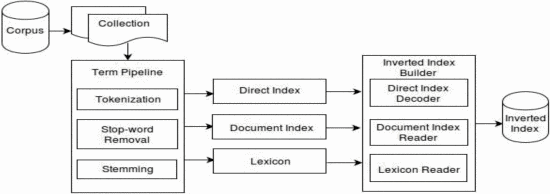
\includegraphics[width=\textwidth]{data-indexing.png}
    \caption{Data Indexing Process \cite{7830087}}
    \label{fig:data-indexing}
\end{figure}

With respect to information retrieval and recommendation system, data indexing has the following benefits:
\begin{itemize}
    \item improves performance in retrieving relevant documents
    \item optimizes the speed of the information retrieval system.
    \item helps to keep the data unique and drop the duplicates
    \item text-based indexes make it easier to search large string values, compared to conventional database approaches.
\end{itemize}

Considering the problem we are solving, data indexing is one of the crucial parts of the implementation strategy. In information retrieval or recommendation systems, latency for fetching the results, the efficiency of results, and relevancy of results for a given problem play the major part of the solution. All these tasks can be easily managed if the data is indexed in an efficient manner. 

\subsection{Elasticsearch and Apache Lucene architecture}
Elasticsearch is built on top of Apache Lucene and uses Lucene indexes. The concept of an inverted index is used while forming an index in Elasticsearch. The inverted index is created by mapping of terms to documents and their position in documents in the form of dictionary \cite{alex2013elastic}.
The dictionaries are sorted, so it's easier to find terms and hence the related documents. Opposite for this is a forward index, where the terms are related to specific documents, which is quite slow in search operations. Hence, an inverted index is used in forming the Elasticsearch index.

For a search operation with multiple terms, it is done by looking up all the terms and their respective occurrences, and the final results are comprised are some form of an aggregate of these results.
The main logic for search operation is, to find the respective terms, then the matching occurrences,  positions and consequently the documents. 

An Elasticsearch index is crated with one or more shards, that can have zero or more replicas. Each shard in an individual Lucene index. Thus, Elasticsearch index is made up of multiple Lucene indexes, which are made up of multiple index segments \cite{alex2013elastic}. A search operation in Elasticsearch index is executed on all the shards, and consequently all the segments and finally merged to give the output. A similar process is followed when multiple indexes are searched. It can also be thought as searching two indexes with one shard is same as searching one index with two shards, in both the cases two Lucene indexes are searched. Elasticsearch is also very flexible and provides options to optimize results, by providing options to define Elasticsearch indexes, which shards(and replicas), the search is directed to. Also, there are options to define index patterns, index aliases, document and search routes, data partitioning and data flow strategies. Figure \ref{fig:elasticsearch-architecture} summarizes this concept and shows the Elasticsearch architecture.

\begin{figure}
    \centering
    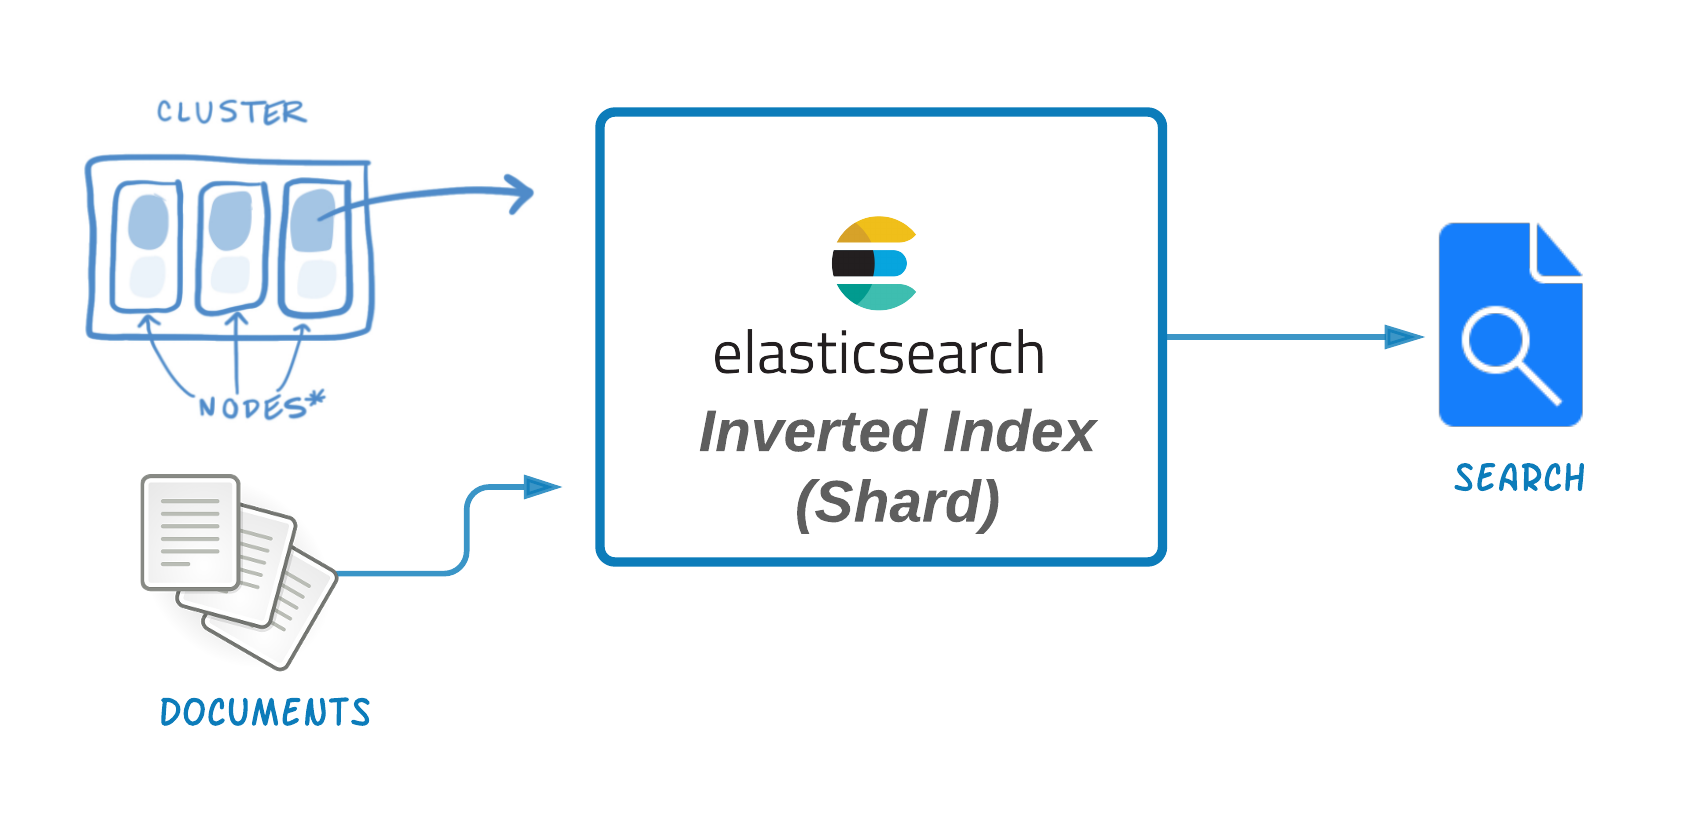
\includegraphics[width=120mm,scale=0.5]{elastic-architecture.png}
    \caption{Elasticsearch Architecture}
    \label{fig:elasticsearch-architecture}
\end{figure}

\subsection{Our implementation in Elasticsearch}
We have used Python and Elasticsearch to manage this task of data indexing. Since Elasticsearch is developed for the purpose of text-based retrieval system, so the major task of efficient indexing is done by it's internal processing. The python script takes care of the data collection, preprocessing and feeding the Elastic server with the data in the right format and remaining part of indexing is done by Elasticsearch. Figure \ref{fig:elasticsearch-architecture} explains the architecture for data indexing process. Once the data is indexed, it is shown as key-value pairs and also retrieved in the same key-value manner (as shown in Figure \ref{fig:citeulike-dataset}). 


The first index for all three datasets is created with the same mapping structure as given in the JSON files. The regular indexing in Elasticsearch stores the term with standard metrics. An important part to note is, all the metrics such as term frequency, document frequency, document length, average document length, etc. are calculated at the time of indexing itself and stored as index metadata. This also plays a significant role in document retrieval since term weights are just fetched from the metadata instead of calculating it at the moment. 

\section{Term Age Calculation and Indexing}
We have created three indexes for every dataset. First is the standard index with all standard metric as explained in the last section. For the second index, we add time normalized term weight factor or the term age to be stored along with other metrics. For calculating the term age, the following steps are done:
\begin{itemize}
    \item Iterate over the IDs stored in the first index and fetch the main article text
    \item Consider the article text of the document and split it into individual words. 
    \item For each of this word, get the origin year that is the year of the first occurrence of this word from etymonline.com.
    Figure \ref{fig:etymonline} shows the search results from the site and \textit{"1660"} is the considered as year of origin for this searched term \textit{"monologue"}.
    \begin{figure}[h!]
    \centering
    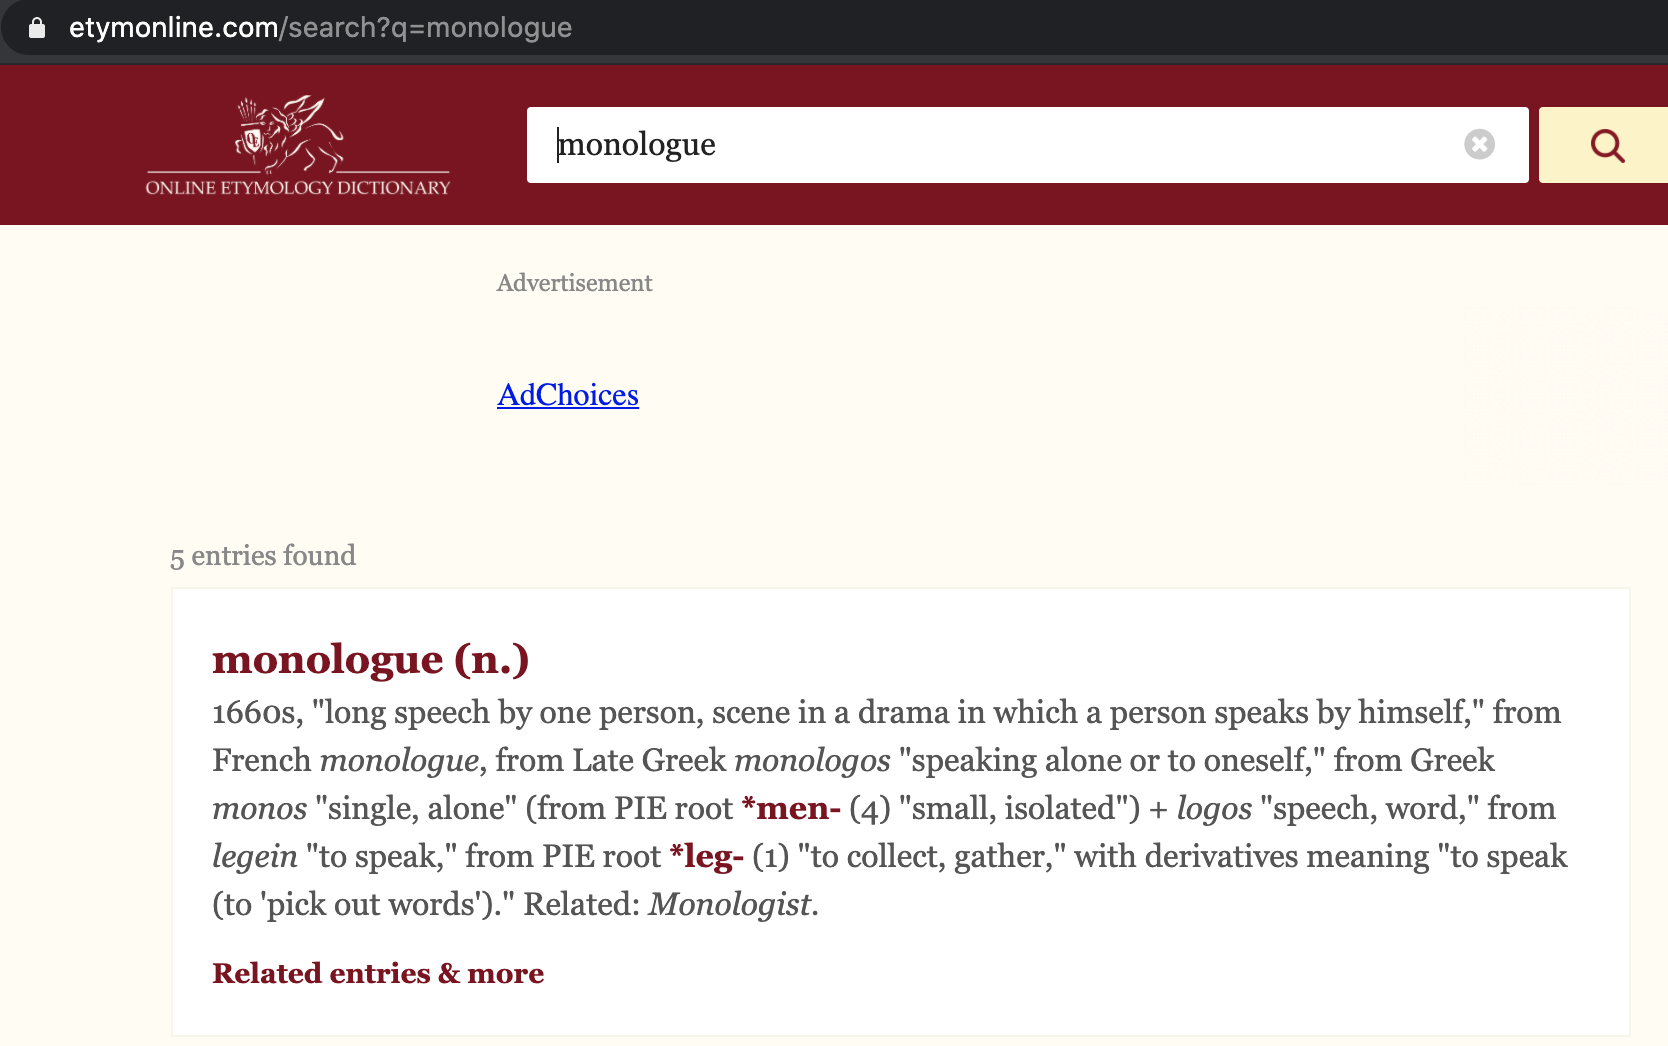
\includegraphics[width=140mm,scale=0.7]{Etymonline.png}
    \caption{Search results from Etymonline}
    \label{fig:etymonline}
    \end{figure}
    \item Calculate the difference in the number of years from the year of the first occurrence, to the current year. We have assumed the base year for our corpus to be 2017(TREC News), 2015(Web AP) and 2019(CiteULike) since that is the year of latest publications. This has been done for uniform term weighting across the corpus and to get the metric unit as documents per year.
    \item Now we fetch the document frequency, $df_{w,D}$ for a specific term $w$ and divide the document frequency with the year difference, as explained in chapter 4. 
    Since the value is relatively large, we have taken its logarithm value to normalize this term. Also, to avoid divide by zero error in cases when the term is newly devised and origin year is the same as the current year, we have added one to the denominator.
    \item Finally, the absolute value of the calculation done in the last step is the term age parameter and is calculated for every term in the article text. 
\end{itemize}

Once we have calculated the term age, we append this along with the terms using a separator. And the newly created article text is indexed in the form of payload index. Since the term age parameter does not have any standard column designated for it, we store it as payloads in the index and later use it in retrieval and relevance score calculation. Updated document text looks like this: \textit{“Americans|5.432 to|0.000 rate|5.466 their|1.080 ideology|3.303 on|0.000 a|0.000 scale|3.455 of|0.000 1|0.000 to|0.000 5|0.000.” }
An important part to note is, that not every term is given a term weight, this happens for a couple of reasons. First, if the origin year could not be traced for the term, this usually happens for proper nouns. Second, if the terms are most frequently used terms such as articles, prepositions, etc., that have a high document frequency value and in result might bias the results of the search query. Figure \ref{fig:payload-index} shows the mapping structure of a payload index, highlighting the term\_vector and analyzer fields showing the added analyzer for payloads.

\begin{figure}[h!]
    \centering
    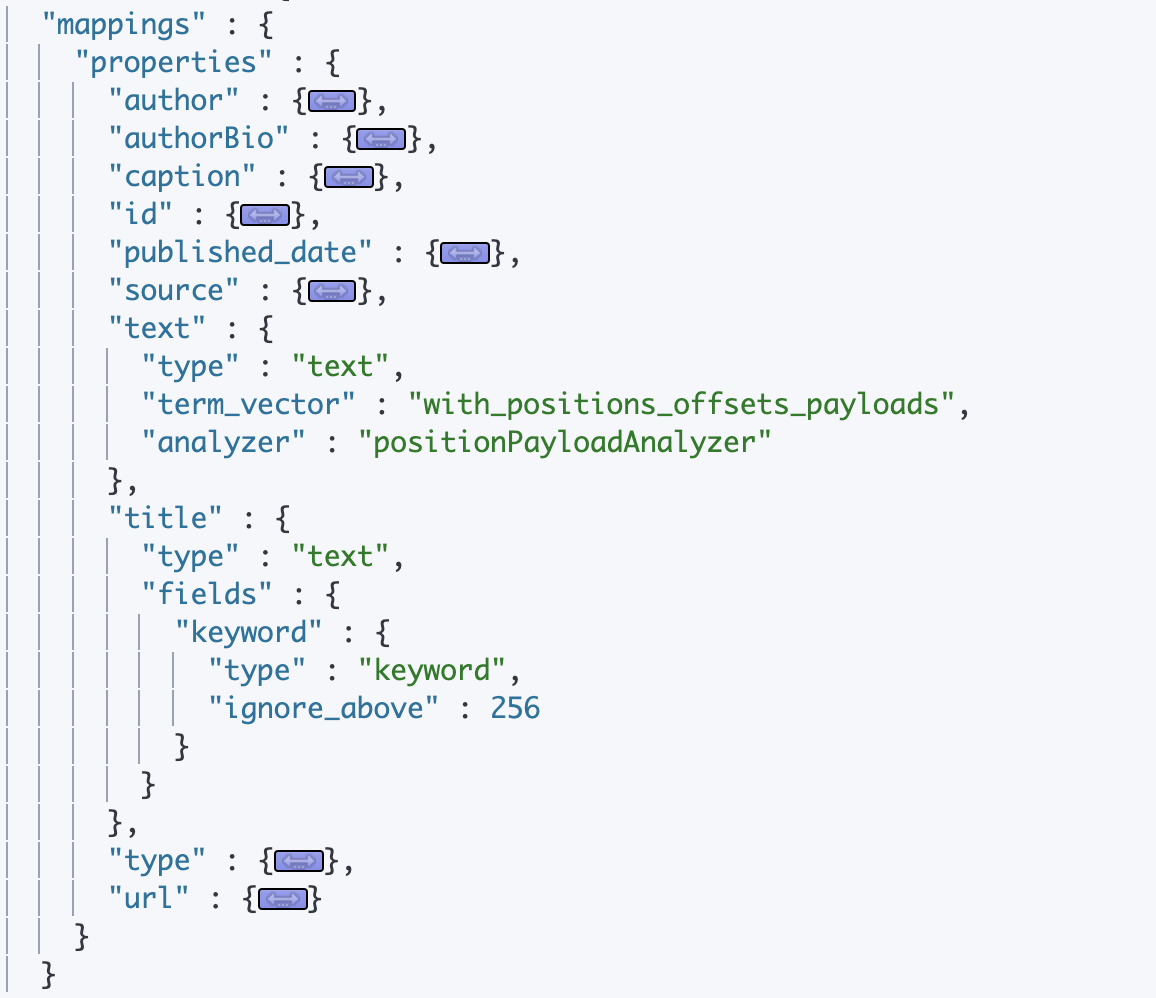
\includegraphics[width=120mm,scale=0.5]{payload-index.png}
    \caption{Payload Index Mapping Structure}
    \label{fig:payload-index}
\end{figure}

\section{USE based Payload Indexing}
For standard term weighting schemes, the relevant documents that are retrieved are based on the most number of term matches with the input query. However, to improve the search results, there are cases when the number of matching terms are less but still, the document might be relevant to the input query considering the semantic context. To overcome this issue and improve the performance of search engine or recommendation system, text embedding models are used, that encodes the text or sentence into a high dimensional numeric vector. These vector representations are developed in a way to consider the linguistic context of the terms into consideration. 

For a good text embedding model, different directions of the vector are coupled with different contexts of the same term. For example, the vector for the term "Canada", will be close to "France" or "French" in one direction and close to "Vancouver" in another direction \cite{julie2019USE}.

Mainly text embedding models focus on the word embedding and encode only the word into a dense vector. However, recently, some advance researches have also started to focus on longer texts such as sentence and try to capture the essence of the sentence into the dense vector. This is usually done with the help of neural network architectures focusing on the semantic context for the terms and sentences. Various advanced embedding models such as  Universal Sentence Encoder (USE) \cite{RN32}, Google’s BERT  \cite{DBLP:journals/corr/abs-1810-04805}, InferSent \cite{DBLP:journals/corr/ConneauKSBB17}, etc. are used for this purpose.


In our research, we have used Universal Sentence encoder model and created an index to store the dense vectors as well as the term age payloads. We have used a pre-trained Tensorflow model to form the dense vectors \cite{google2018use}. We use the following method to create a USE based index :
\begin{itemize}
    \item Iterate over the IDs stored in the first index and fetch the main article text.
    \item Main article text is run through a pre-trained Tensorflow model, creating a 512 dimension vector for the main text.
    \item Term age parameter is calculated in the same way as explained in the last section
    \item Same model is used to compute the dense vector for input query at the time of text retrieval.
\end{itemize}
Figure \ref{fig:architecture} shows the high-level architecture of the created indices, and search application.
Figure \ref{fig:use-index-mapping} shows the mapping structure of USE based index highlighting thee dense vector of 512 dimensions.
\begin{figure}
    \centering
    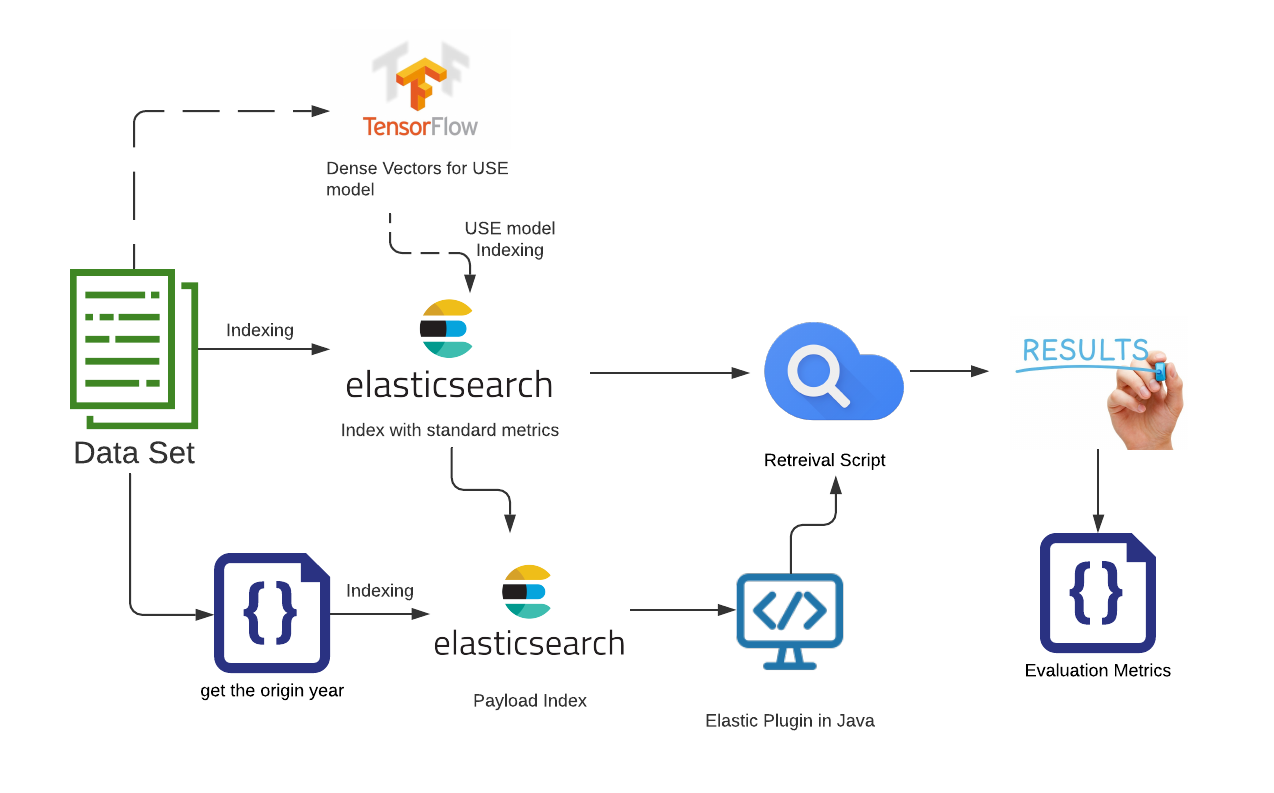
\includegraphics[width=140mm,scale=0.7]{System Architecture thesis.png}
    \caption{System Architecture}
    \label{fig:architecture}
\end{figure}

\begin{figure}[h!]
    \centering
    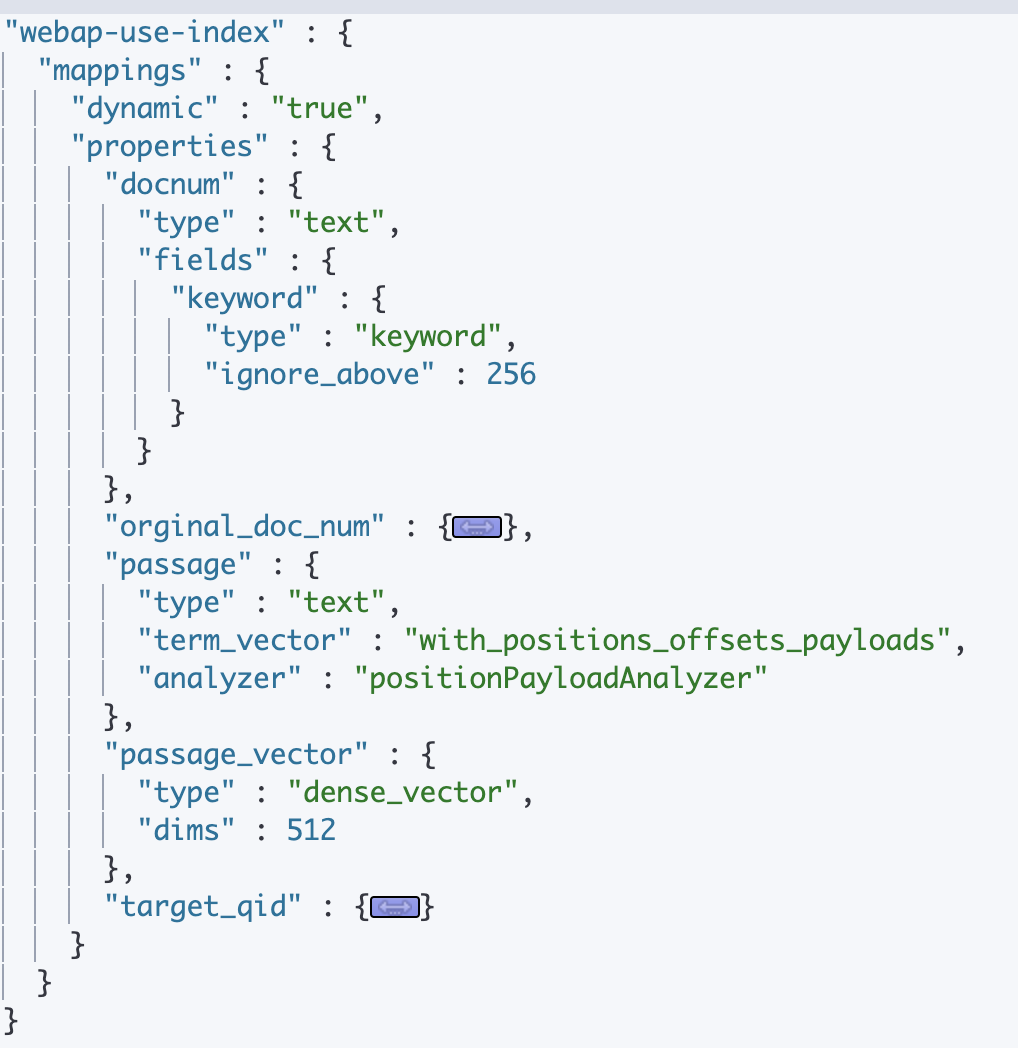
\includegraphics[width=120mm,scale=0.4]{use-index.png}
    \caption{USE based payload Index mapping}
    \label{fig:use-index-mapping}
\end{figure}

\section{Implementing Relevance Score calculation}
We have used Elasticsearch to create all three different indices for our datasets. Since Elasticsearch is built on top of Apache Lucene, that uses multiple parameters for score calculation. To have a uniform comparison with the baseline models we have implemented two different plugins. The first one just fetches standard metrics such as TF, IDF, Document length, etc. to calculate the relevance scoring and retrieves the results. The second plugin scores based on the calculated term weight parameter along with the standard metrics. These plugins are developed in Java and based on Apache Lucene plugins library. These plugins are then added into the Elasticsearch installation and also specified while indexing documents. Finally, we compare the results retrieved for the given set of queries from both these executions to our ground truth results. 

\subsection{Implementing Time Normalized TF-IDF(tTF-IDF)}
For standard TF-IDF model, it is based on just two metrics, Term frequency and inverse document frequency. These metrics are already stored in the metadata of the index are just fetched directly while retrieving documents. The formula for TF-IDF is given in equation \ref{eq:5.4}.
\begin{equation} \label{eq:5.4}
        wt_{w,d} = tf_{w,d}*log(\frac{N}{df_{w,d}})   
\end{equation}  
We fetch the results from the first index using this standard metric calculation and forms the first set of our results for the given input queries. For second set of results, we fetch the results based on our extended version of formula given in equation \ref{eq:5.5}. This is titled as tTF-IDF, where extra t stands for temporal dimension added to the existing formula. The term age parameter $t_{w,D}$ is stored as the term payload in the documents metadata. We leverage this metadata in our plugin to formulate this and calculate the relevance scores for the documents retrieved.
\begin{equation} \label{eq:5.5}
        wt_{w,d} = t_{w,D}*tf_{w,d}*log(\frac{N}{df_{w,d}})   
\end{equation} 
The results retrieved by using this updated formula, forms our second set of results. We have then compared the first and second set of results based on the precision, recall, F1 and NDCG metrics discussed in detail in chapter 7.

\subsection{Implementing Time Normalized BM25(tBM25)}
BM25 model is also based on term frequency and inverse document frequency, but the calculation logic for both these metrics is different from the standard TF-IDF model. IDF calculation is mainly the same, with just an added 1 in the denominator to avoid divide by zero exception. For TF, there are some added metrics of field length and average field length that are used. The term weight calculation is shown in equation \ref{eq:5.6}. 

\begin{equation} \label{eq:5.6}
    wt_{w,d} = \sum_{i}^{n}IDF(q_{i}) * \frac{f(q_{i},D)*(k1+1)}{f(q_{i},D)+k1*(1-b+b*\frac{fieldLen}{avgFieldLen})}
\end{equation}
First set of results for BM25 are fetched using this standard calculation. For second set of results, we fetch the results based on our extended version of formula given in \ref{eq:5.7}. This is titled as tBM25, where extra t stands for temporal dimension added to the existing formula. The term age parameter $t_{w,D}$ is stored as the term payload in the documents metadata. We leverage this metadata in our plugin to formulate this and calculate the relevance scores for the documents retrieved.
\begin{equation} \label{eq:5.7}
    wt_{w,d} = \sum_{i}^{n} t_{w,D}*IDF(q_{i}) * \frac{f(q_{i},D)*(k1+1)}{f(q_{i},D)+k1*(1-b+b*\frac{fieldLen}{avgFieldLen})}
\end{equation}

\subsection{Implementing Time Normalized Universal Sentence Encoder(tUSE)}
For a USE based model along with text similarity search, we have used cosine similarity function. Cosine similarity is already integrated in Elasticsearch and we leverage the same while getting the results. For this model, the input text query is first run through the same pre-trained sentence embedding model that produces a numeric vector. Now, to calculate the relevance score, we calculate the vector similarity between the input vector and the dense vector of the indexed documents. Cosine similarity calculates the angle $\theta$ between the two given vectors. This formulation is given in \ref{eq:5.8}.
\begin{equation} \label{eq:5.8}
    \cos \theta = \frac{\sum_{1}^{n} \vec a_{i}b_{i}}{\sqrt{\sum_{1}^{n} \vec a_{i}^2}\sqrt{\sum_{1}^{n} \vec b_{i}^2}}
\end{equation}
Some of the example, showing how this model return results are:
\begin{itemize}
    \item "zipping files" will also return results like "compression of files"
    \item "convert int to double" will also return results like "translate int to float numbers"
\end{itemize}
Although, there is not a strong overlap of terms in the input and output, still the results are considered relevant based on the semantics.

This forms the standard first set of results for our given input queries. As done in the previous models, we multiply the term age factor(stored in the metadata payload) in the standard calculation to get the tUSE formula as shown in equation \ref{eq:6.9}.
\begin{equation} \label{eq:6.9}
    \cos \theta = t_{w,D}*\frac{\sum_{1}^{n} \vec a_{i}b_{i}}{\sqrt{\sum_{1}^{n} \vec a_{i}^2}\sqrt{\sum_{1}^{n} \vec b_{i}^2}}
\end{equation}


\section{Key challenges}
In implementing and formulating this research project, we encountered some challenges listed below:
\begin{itemize}
    \item Finding an openly available ground truth dataset that matches up requirements was challenging. There are many text-based datasets available on the web, but a lot less with the defined gold standard. Even for the available ones, finding out the temporal context and how to apply it was challenging.
    \item Although Elasticsearch is open source and used in multiple research and production environments, there is still very less information available for defining payload index and how to use its scoring methodology. Figuring out the way to include time factor along with the index was one of the major roadblocks in implementing this research. We tried multiple methods such as using term age as boost parameter while querying, indexing term age as a separate dense vector field in the index, using a script score and function score methods in elasticsearch.  But none of them sufficed to our research statement.
    \item The existing libraries in Python for Precision and NDCG do not give out the correct results as per the metric definitions. For example, on using scikit-learn's NDCG function returns the NDCG value as 1, even when no results match in the result set. To overcome this issue, we implemented custom-built methods for computing NDCG and precision for our algorithm and validated it giving the correct results as per the metric definition.
    
    
\end{itemize}

  \chapter{Results and Discussion}
\section{Precision, Recall and F1 Scores Comparison}
In 2 out of 3 algorithms, our term-recency modification improved the performance notably. When measured by p@10, tTF-IDF outperformed TF-IDF by an average 47\% and tUSE outperformed USE in 2 of the 3 datasets by average 14.3\% but performed 50\% worse in the third dataset (shown in Figure \ref{fig:tf-idf-precision-comparison} and \ref{fig:use-precision-Comparison}). The time normalized BM25 version, however, performed 32\% worse than BM25 (shown in Figure \ref{fig:bm25-precision-comparison}). 


In the general case of Information retrieval evaluation, Recall and F1 measures give different results than precision metrics, if the given number of relevant results are not fixed. In our datasets, only TREC news has a varied number of relevant results given as ground truth. In other cases, if the number of given relevant results are constant, then all three values, that is precision, recall and F1 scores remain the same. 
In case of TREC news dataset, for calculating the recall and F1 scores, we fetch the top 100 results for the given query sets. For uniformity in the metric calculation, we compute the precision scores as well. The result metrics are shown in \textit{Figure \ref{fig:recall-f1-metrics}}. Recall and F1 scores as well show a significant improvement of time normalized models over the standard ones. Evaluating in terms of recall, we see a 93\% improvement in the tTF-IDF model over TF-IDF and a 28\% improvement in tUSE model over the USE model. While tBM25 performed 27\% worse than the standard BM25 model.

\begin{figure}
    \centering
    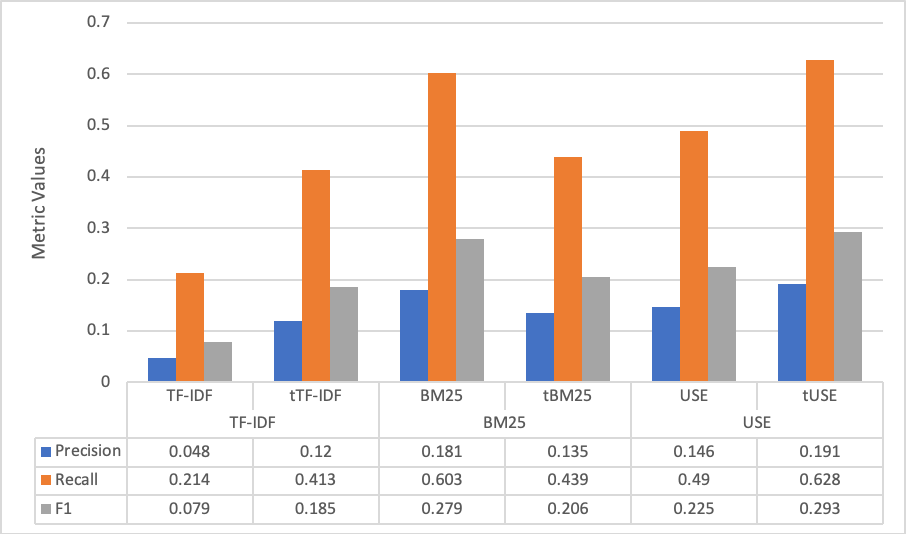
\includegraphics[width=\textwidth]{recall-f1scores.png}
    \caption{Precision, Recall, F1@100 scores for TREC News }
    \label{fig:recall-f1-metrics}
\end{figure}

\subsection{tTF-IDF vs TF-IDF}
On comparing in terms of precision and NDCG scores, tTF-IDF model outperformed TF-IDF model in all three datasets. Digging deep into the results, for TREC news dataset, we see a massive improvement of 115\% in the precision score. While for CiteULike tTF-IDF outperformed TF-IDF by 11\% and for WebAP dataset, tTF-IDF outperformed by 15\% (shown in Figure \ref{fig:tf-idf-precision-comparison}).
Based on the study of corpus and results retrieved for each dataset, the following inferences can be derived:
\begin{itemize}
    \item presence of temporal context in a news corpus is high compared to other text corpora. The reason for such an assumption is that news highlights events of a different era, having a higher chance of showing time relation compared to any other text
    \item Size of the corpora is different and so the variation in the term age is another factor. Since the term age is also dependent on the document frequency, so the size of corpus also affects the term age indirectly.
    \item Term age might not be adding much relevance to CiteULike and WebAP dataset, but performs significantly well to introduce the term age for improving results. And the results could be improved by testing out with different normalization factors for term age as well as tTF-IDF.
\end{itemize}
\begin{figure} [h!]
    \centering
    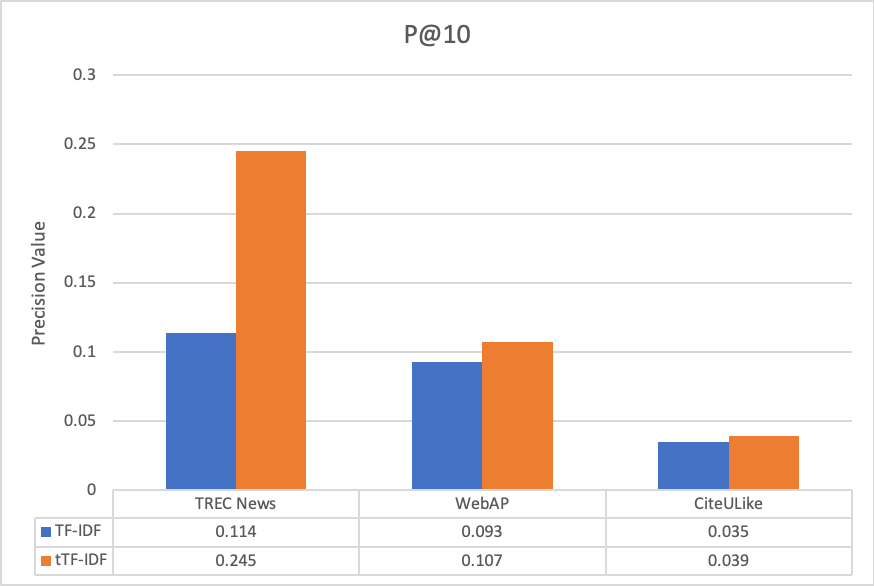
\includegraphics[width=120mm,scale=0.5]{p-10-tf-idf.png}
    \caption{TF-IDF vs tTF-IDF Precision Comparison}
    \label{fig:tf-idf-precision-comparison}
\end{figure}
\subsection{tBM25 vs BM25}
Time normalized BM25 model did not perform well for any of the datasets. tBM25 model performed 9.4\% worse for TREC news dataset, 44\% worse for CiteULike dataset, and 42.8\% worse for the Web AP dataset (shown in \ref{fig:bm25-precision-comparison}).
On closer analysis of the BM25 model, we see 27 out of 50 queries in TREC news task, gave better or almost similar results in case of time normalized BM25 model when compared to the classic approach. Assuming that the news text has a temporal context in them, these results are also promising and need to be worked upon for improvised results in future work.
Based on the results retrieved and study, the following inferences can be derived for tBM25 model:
\begin{itemize}
    \item BM25 and tBM25 model performs better than the classic TF-IDF and tTF-IDF model for all cases. 
    \item current term age formulation is not improvising the BM25 search algorithm. Different term age formulation or normalization factors need to be tested to verify the significance of term age in the BM25 algorithm.
    \item The reason for the worse performance of tBM25 model can also be because of the additional metric field length and average field length used in the BM25 formula. It might be possible that the current term age formulation does not fit in well with the field length metrics.
    \item Tuning of other constant parameters in BM25 formula, that is k1 and b can also be tried to improvise upon the tBM25 model.
\end{itemize}
\begin{figure} [h!]
    \centering
    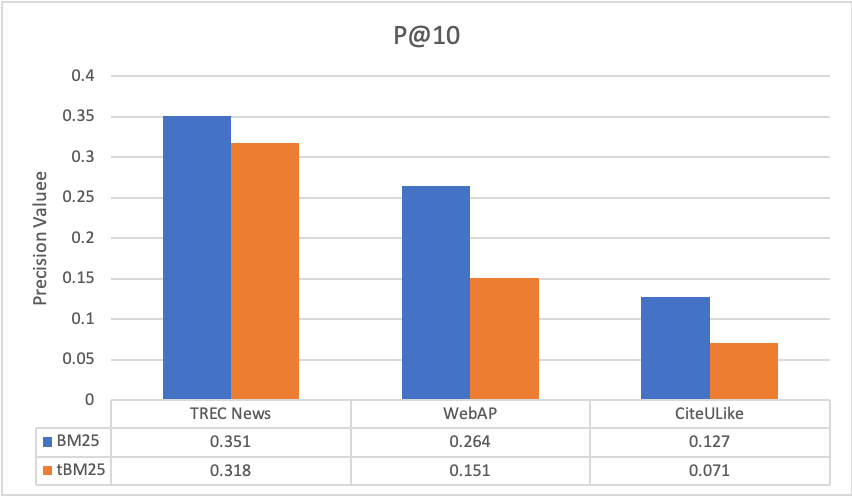
\includegraphics[width=120mm,scale=0.5]{p-10-bm25.png}
    \caption{BM25 vs tBM25 Precision Comparison}
    \label{fig:bm25-precision-comparison}
\end{figure}
\subsection{tUSE vs USE}
Time normalized Universal Sentence Encoder(tUSE) model outperformed the USE model in 2 of the 3 datasets. For TREC News dataset we observed 18\% improvement in tUSE model over standard USE. And in CiteULike, we get a 10.67\% improvement in the time normalized version. While it performed 50\% worse for the Web AP dataset. 

Analyzing the tUSE model in WebAP dataset, we see it does not perform well against the USE model. One of the possible reasons for this might be the size of the corpus used, that is, TREC news corpus has approximately 600k documents while Web AP dataset has just 6k documents, which is 100 times less than the former dataset. However, this is an inference based on the results retrieved and has not been verified. There might be other possible reasons, such as the size of documents, size of queries used, number of proper nouns in the queries, etc. Or probably term age might not be a relevant metric for this dataset. These possible reasons still need to be analyzed before affirming out a conclusion on these contrasting results.

Based on the study of corpus and results retrieved for each dataset, the following inferences can be derived:
\begin{itemize}
    \item out of TF-IDF, BM25, and USE, USE model performs best for fetching results for queries in the English language. And apparently, tUSE model performs better for 2 of the three datasets.
    \item currently implemented time normalization does not work well with the Web AP dataset in case of USE based relevance scoring.
    \item For background linking task in TREC news dataset, USE gave a p@10 value 0.52 while tUSE gave p@10 value of 0.614, which is far better compared to TF-IDF(0.114) and tTF-IDF(0.245). From this observation, it is evident that the semantics-based search is more promising than keyword-based search for such tasks.
\end{itemize}
\begin{figure} [h!]
    \centering
    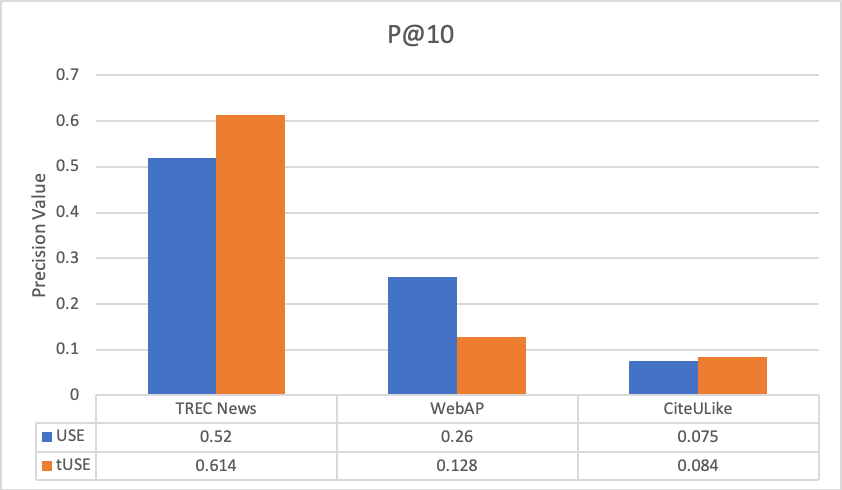
\includegraphics[width=120mm,scale=0.5]{p-10-USE.png}
    \caption{USE and tUSE Precision Comparison}
    \label{fig:use-precision-Comparison}
\end{figure}
\section{NDCG Score Analysis}
NDCG is used to evaluate the ranking measure of the results retrieved. we have used the top 10 results to validate the NDCG scores. And NDCG@10 leads to similar results as seen for precision@10, illustrated in section 7.1. We have calculated the NDCG scores only for TREC News and WebAP datasets, for CiteULike dataset, NDCG cannot be calculated, since this is based on the references used in the research paper and there is no ranking specified for the citations. 
For TREC news, we see tTF-IDF outperformed TF-IDF by 59\% and tUSE outperformed USE model by 10.76\%. While for tBM25 performed 18.3\% worse than the BM25 model. These comparison results are shown in figure \ref{fig:ndcg-scores}. 
Based on these NDCG scores and the p@10 metrics, it is evident that time normalized models are promising and have a wide scope of applications in information retrieval and recommendation systems.


\begin{figure}
    \centering
    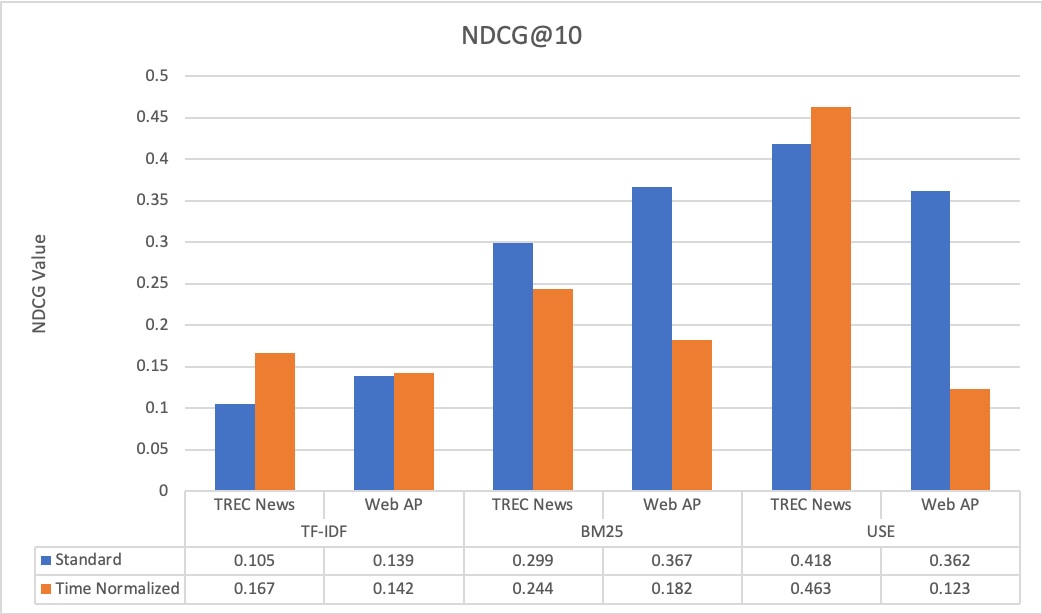
\includegraphics[width=\textwidth]{ndcg-comparison.png}
    \caption{NDCG@10 Score Comparison}
    \label{fig:ndcg-scores}
\end{figure}


\section{Term Age Distribution Analysis}
Looking at the distribution of words and their origin years, we observe a vast range of origin ranging from the year 1100 to the year 2015, illustrated in Figure \ref{fig:origin-year-distribution}. Most of the terms used are in the year range of 1800-1900, followed by year range 1500-1600. For TREC news dataset, we observed the document frequency ranges from 2 to 550k. Combining both of them, we get the term age ranging from 0 to 9.71, with a mean of 0.9308 and median of 0.1568. 
Similarly for other datasets, we observed a similar pattern of origin year but a change in the document frequencies. And consequently, variation in the term age is observed in the CiteUlike and Web AP dataset.Distribution Statistics for term age is shown in Table \ref{table:7.1}.

\begin{table}[h!]
\centering
\begin{tabular}{ |c|c|c|c|c|c|c| }
 \hline
 \textbf{Min.}	& \textbf{Mean} & \textbf{3rd quartile} & \textbf{Max.} & \textbf{Median} & \textbf{Std. dev.} & \textbf{Variance}\\
 \hline
 0 & 0.9308 & 1.5198 & 9.7120 & 0.1568 & 1.3363 & 1.7856 \\
\hline
\end{tabular}
\caption{Term Age Distribution}
\label{table:7.1}
\end{table}


\begin{figure}
    \centering
    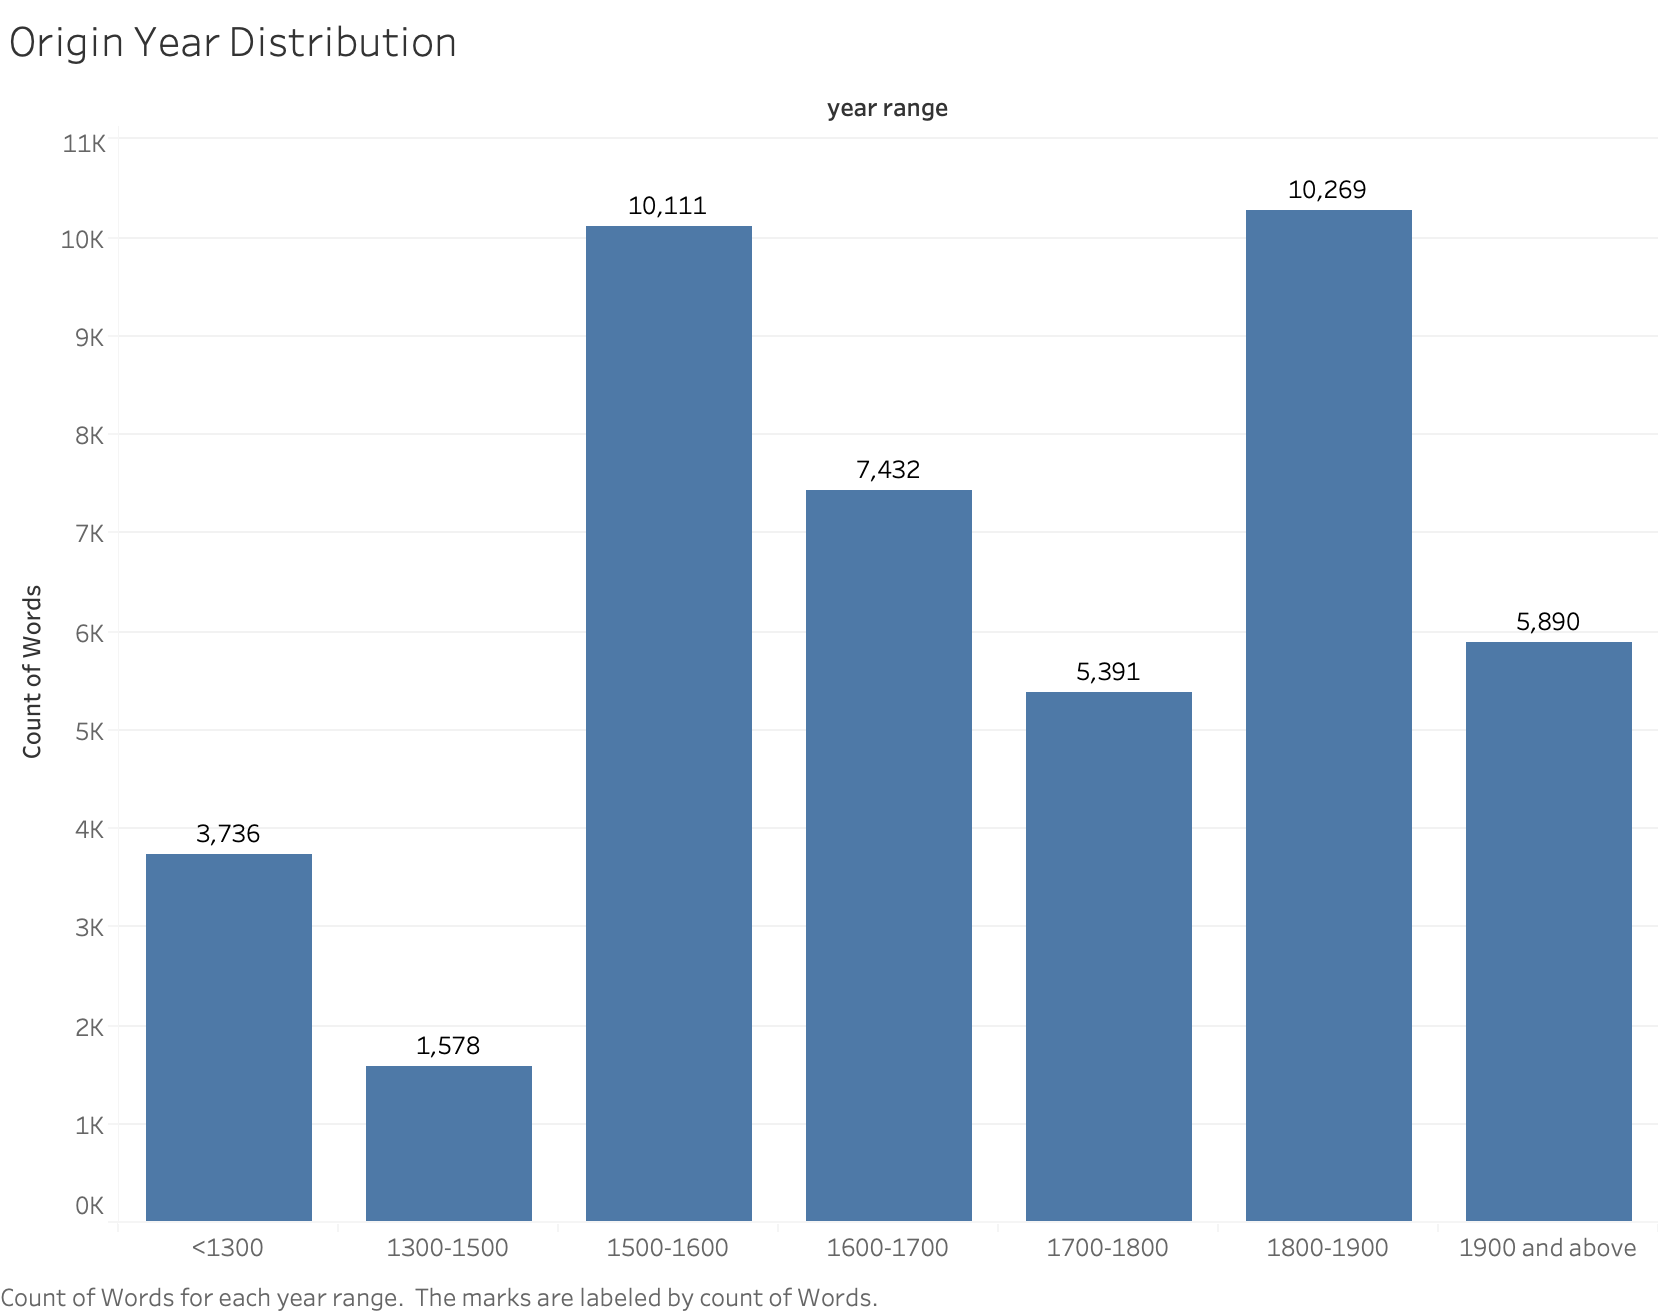
\includegraphics[width=100mm,scale=0.7]{origin year distribution.png}
    \caption{Origin Year Distribution in years}
    \label{fig:origin-year-distribution}
\end{figure}

\begin{figure}[h!]
    \centering
    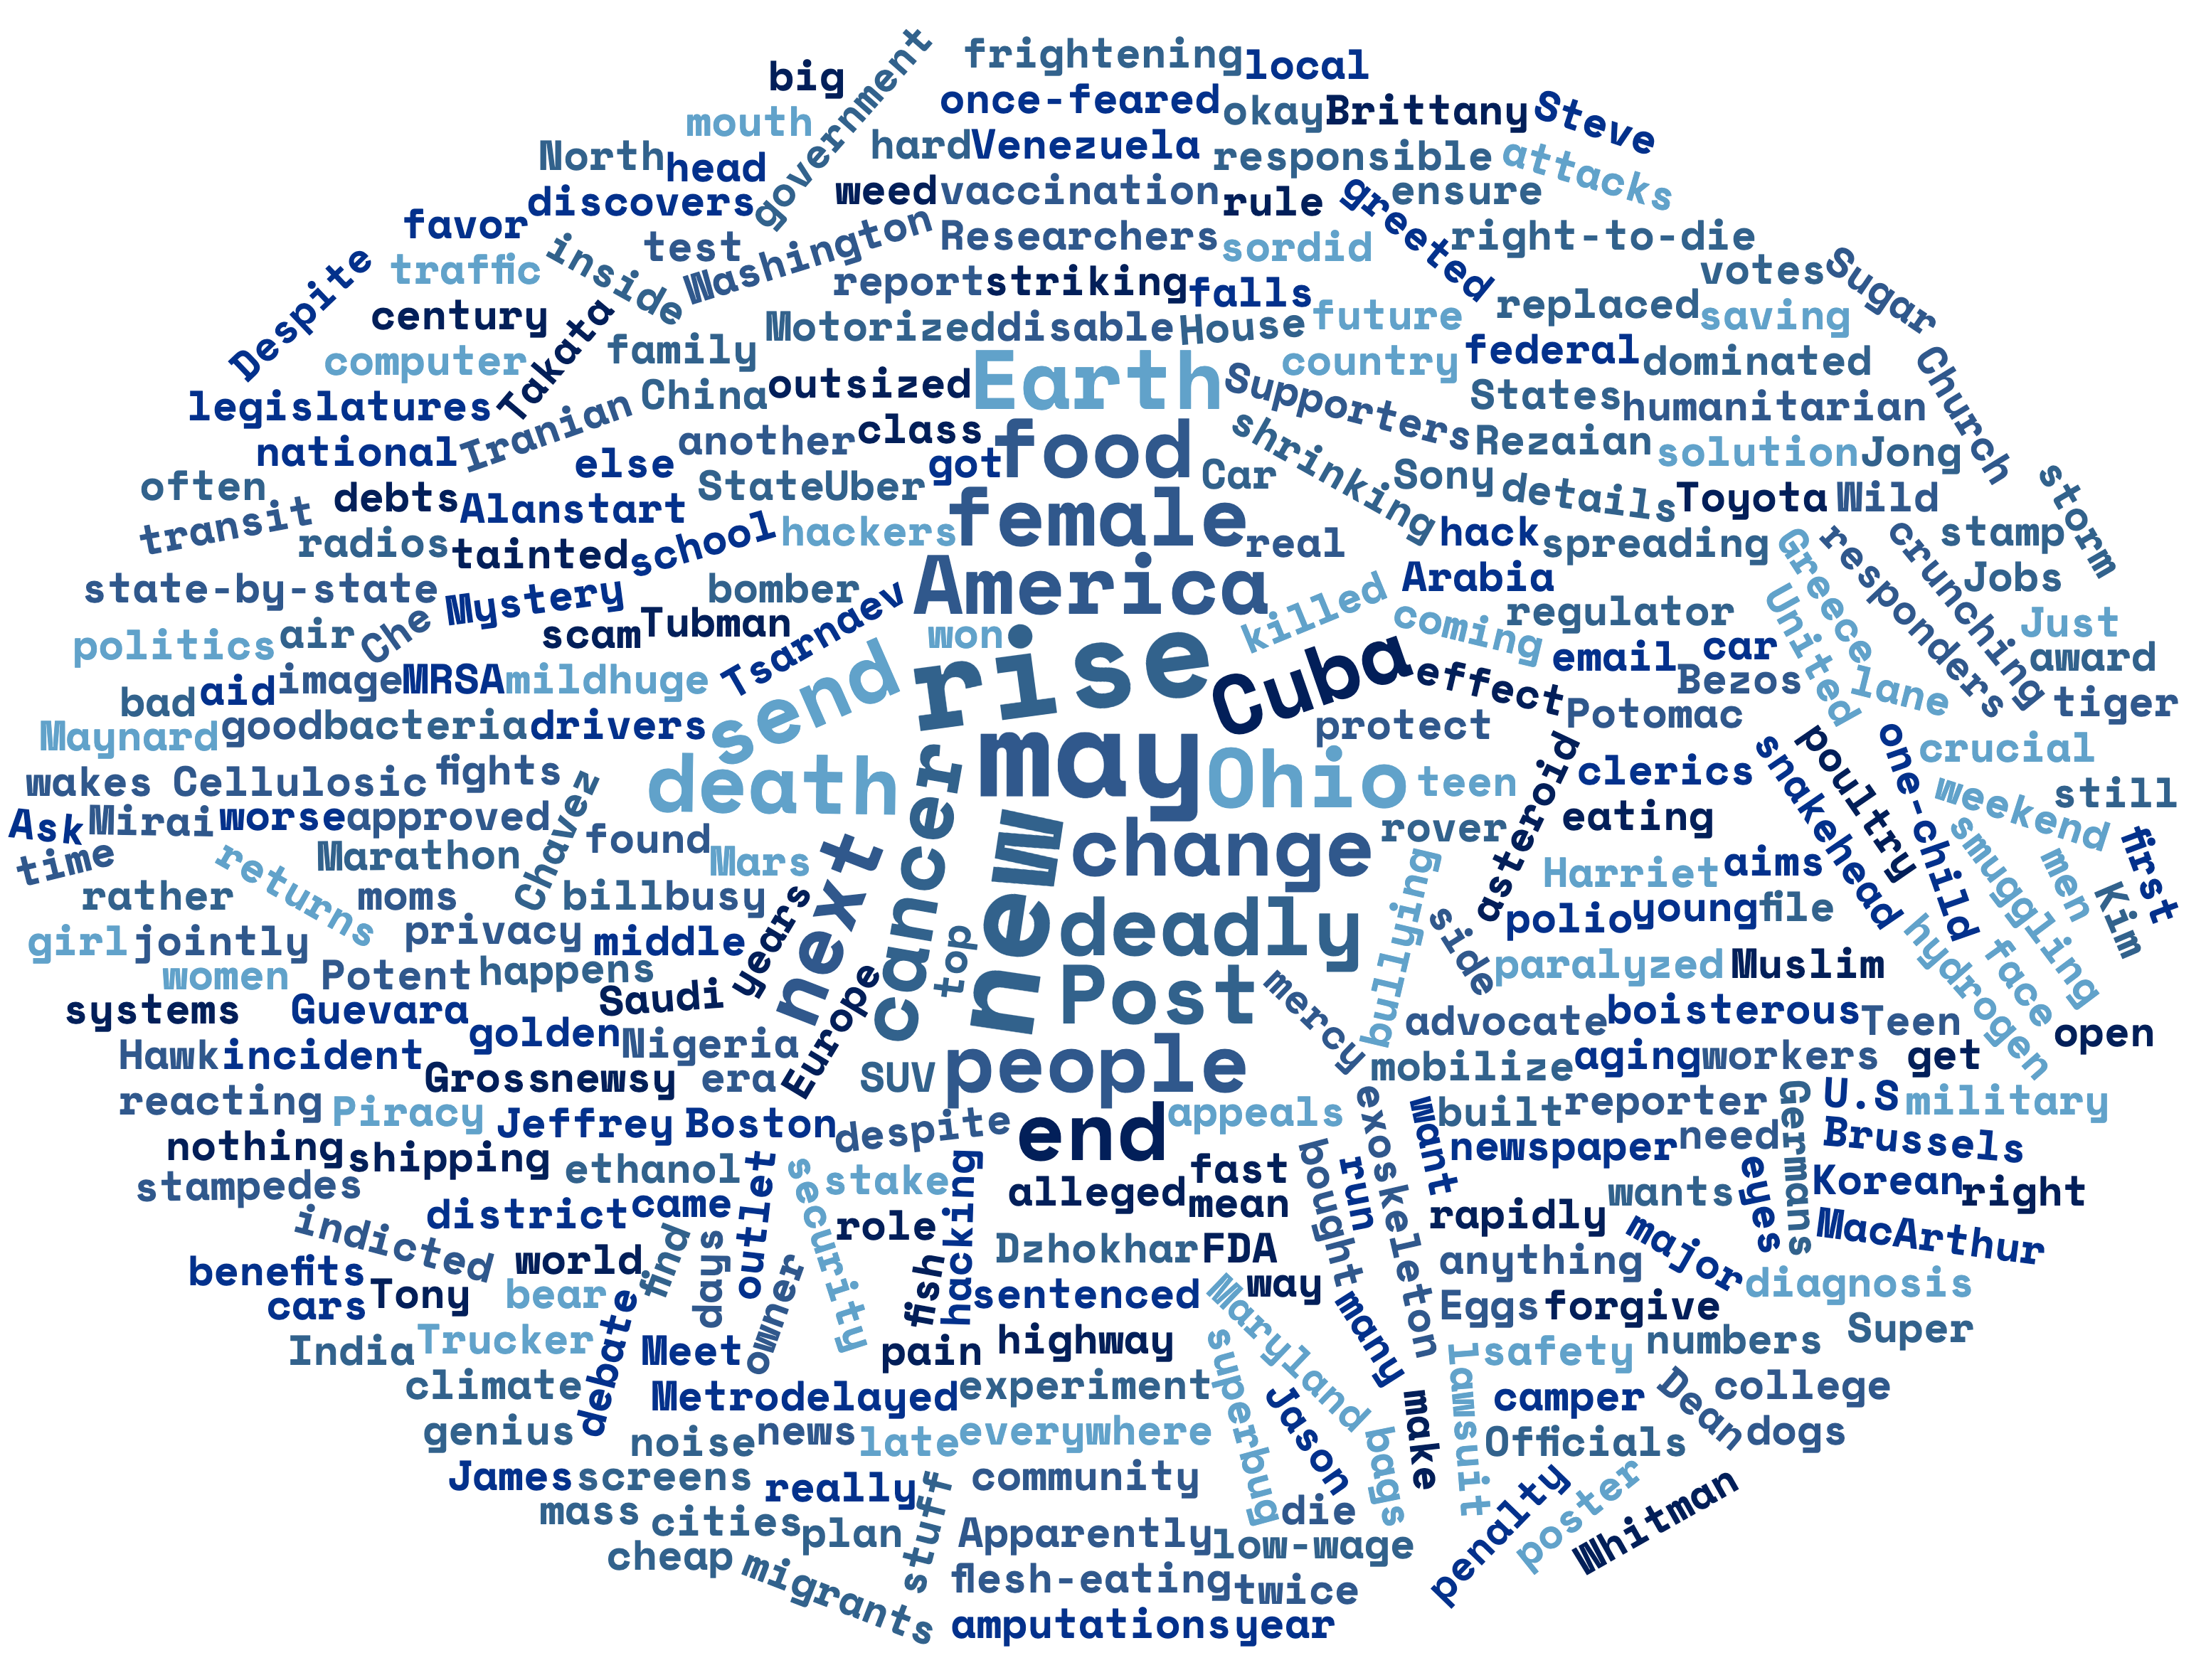
\includegraphics[width=140mm,scale=0.5]{searched-wordcloud.png}
    \caption{Searched words cloud in TREC News Dataset}
    \label{fig:search-word-cloud}
\end{figure}

Another interesting statistic to look at is the searched words and their frequency of search. We did analyse the searched terms pattern in for the TREC news background linking task and a word cloud for the searched words is shown in Figure \ref{fig:search-word-cloud}. In the word cloud, the size of the term shows the frequency of the term used. Most frequent terms in the search queries are, 'America', 'Cuba', 'Ohio', 'Change', 'deadly', 'rise', 'new', 'death', cancer', 'female', 'food', 'Earth' and some more terms that are shown in Figure \ref{fig:search-word-cloud}. 
  \chapter{Conclusion and Future Work}
\section{Conclusion}
In this research, we proposed a novel algorithm for term weighting. The presented approach shows the significance of temporal distribution along with existing space distribution of terms. We suggest the scheming of a term recency parameter based on the origin of the word and the usage in the document corpus. This factor is used along with the standard weighting values (such as TF and IDF) for relevance scoring in the information retrieval system. The time normalized algorithm suggested is a robust model, that can fit into multiple use cases. The origin year used in the term age calculation can be traced to various sources as per the problem statement. The algorithm is tested on a news dataset, with queries trying to find links with the documents, Web answer retrieval dataset and research papers citations dataset. We implemented this on top of standard term weighting methodologies, TF-IDF, BM25 and Universal Sentence Encoder models.

Experiments conducted on the search relevance system show that term-recency based TF-IDF and tUSE model outperforms the classic TF-IDF and classic USE algorithms with a significant margin when measured in terms of average precision, recall, F1 and NDCG. 
With these significant results, this can be extended to other term weighting methodologies as well. It sets a premise which can be experimented further to several other fields such as user modelling, personalization, recommendations, classification, etc.

\section{Limitations and Future Work}
One of the major drawback of our work was the time-based BM25 model, did not perform well for any of the datasets considered. Time-based BM25 model needs to be analysed in depth to get a better understanding of the limitation and study the introduction of term recency for such models. The possible reason might be term recency is not a valid parameter for BM25 model or the normalization method does not align well with the existing metrics used or we need to check up another normalization or scale. These methods need to be carefully studied to justify the introduction of the term recency parameter in BM25 term weighting.

Another drawback we saw in our existing study was tUSE model did not perform well for the WebAP dataset. We have not done much analysis on the reason for this drop of performance but certain inferences are derived based on the study of the dataset and algorithm. One of the possible reasons for this might be the size of the corpus used, that is, TREC news corpus has approximately 600k documents while Web AP dataset has just 6k documents, which is 100 times less than the former dataset. However, this is an inference based on the results retrieved and has not been verified. There might be other possible reasons, such as the size of documents, size of queries used, number of proper nouns in the queries, etc. Or probably term age might not be a relevant metric for this dataset. These possible reasons still need to be analyzed before affirming out a conclusion on these contrasting results. This part can also be reviewed for a short study and understanding the working of term age-based USE model.

As per our current model, we have introduced an elastic plugin to include the term age parameter indexed as payload in the Elasticsearch indices. However, this way of calculating relevancy scores and fetching results is not a very efficient method of information retrieval. For obvious reasons of adding extra payload and computation, this method retrieves results much slower than the standard way of information retrieval through Elasticsearch. An effective way to reduce latency in fetching the relevant results can also be taken up as a part of the future scope for this project.


Another important experiment that can be carried out in the future work is to test out different time normalization and time scaling parameters for calculating term age. We have just tested one normalization based on retrieving term-age as documents per year, that gave out significant results for our tested datasets. These can be extended to study different time normalization factors and there impact on the results fetched. Also, the use of term age parameter in the equation for term weight, like the impact of dividing the factor, or adding some constant to normalize the terms. And a different level of term age, like squaring, square root, etc. can be tested for further analysis on the topic.


We performed our study mainly focused on information retrieval task, however, there are many other applications for term weighting, where term recency can be applied. Term age parameter can be introduced in other tasks such as text classification, user modelling, recommender systems and other related text-based models. Term recency has an ample scope in user modelling space, by building out user models based on the short term contexts and long term contexts. And further using these models for recommendations or improving search results. At this point, this study can be considered as a strong premise for the validation of the term recency model in the term weighting methodology and can be extended for a vast scope.




%\begin{thebibliography}{refs}                   %% Start your bibliography here; you can
\bibliographystyle{ieeetr}
\bibliography{refs}                               %% also use the \bibliography command
%\end{thebibliography}                             %% to generate your bibliography.


%\addcontentsline {toc}{chapter}{Appendices}       %% Force Appendices to appear in contents
%\begin{appendix}
% \include{appendix1}
% \include{appendix2}
% \end{appendix}


%\addcontentsline {toc}{chapter}{Bibliography}     %% Force Bibliography to appear in contents


\end{document}                                    %% END THE DOCUMENT
